%%%%%%%%%%%%%%%%%%%%%%% file template.tex %%%%%%%%%%%%%%%%%%%%%%%%%
%
% This is a general template file for the LaTeX package SVJour3
% for Springer journals.          Springer Heidelberg 2010/09/16
%
% Copy it to a new file with a new name and use it as the basis
% for your article. Delete % signs as needed.
%
% This template includes a few options for different layouts and
% content for various journals. Please consult a previous issue of
% your journal as needed.
%
%%%%%%%%%%%%%%%%%%%%%%%%%%%%%%%%%%%%%%%%%%%%%%%%%%%%%%%%%%%%%%%%%%%
%
% First comes an example EPS file -- just ignore it and
% proceed on the \documentclass line
% your LaTeX will extract the file if required
\begin{filecontents*}{example.eps}
%!PS-Adobe-3.0 EPSF-3.0
%%BoundingBox: 19 19 221 221
%%CreationDate: Mon Sep 29 1997
%%Creator: programmed by hand (JK)
%%EndComments
gsave
newpath
  20 20 moveto
  20 220 lineto
  220 220 lineto
  220 20 lineto
closepath
2 setlinewidth
gsave
  .4 setgray fill
grestore
stroke
grestore
\end{filecontents*}
%
\RequirePackage{fix-cm}
%
%\documentclass{svjour3}                     % onecolumn (standard format)
%\documentclass[smallcondensed]{svjour3}     % onecolumn (ditto)
\documentclass[smallextended]{svjour3}       % onecolumn (second format)
%\documentclass[twocolumn]{svjour3}          % twocolumn
%
\smartqed  % flush right qed marks, e.g. at end of proof
%
\usepackage{graphicx}
\usepackage[ruled,vlined]{algorithm2e}
\usepackage{subcaption} 
\usepackage{amsmath}
%\usepackage{float}
\usepackage{hyperref}
%
% \usepackage{mathptmx}      % use Times fonts if available on your TeX system
%
% insert here the call for the packages your document requires
%\usepackage{latexsym}
% etc.
%
% please place your own definitions here and don't use \def but
% \newcommand{}{}
%
% Insert the name of "your journal" with
% \journalname{myjournal}
%
\begin{document}

\title{Constrained Recommendations for Query Visualizations%\thanks{Grants or other notes
%about the article that should go on the front page should be
%placed here. General acknowledgments should be placed at the end of the article.}
}
%\subtitle{Do you have a subtitle?\\ If so, write it here}

%\titlerunning{Short form of title}        % if too long for running head

\author{Ibrahim A. Ibrahim         \and
        Abdullah Albarak \and %etc.
				Xue Li
}

%\authorrunning{Short form of author list} % if too long for running head

\institute{I. Ibrahim \at
              School of Infornation Technology and Electrical Engineering, University of Queensland, Australia \\
             % Tel.: +123-45-678910\\
              %Fax: +123-45-678910\\
              \email{i.ibrahim@uq.edu.au}           %  \\
%             \emph{Present address:} of F. Author  %  if needed
           \and
           A. Albarak \at
              \email{a.albarrak@uq.edu.au} 
							\and 
							Xue Li \at
							\email{xueli@itee.uq.edu.au} 
}

\date{Received: date / Accepted: date}
% The correct dates will be entered by the editor


\maketitle

%\begin{abstract}
%Insert your abstract here. Include keywords, PACS and mathematical
%subject classification numbers as needed.
\begin{abstract}
%
The improvement of data storage and data acquisition techniques has led to huge accumulated data volumes  in a variety of 
applications.
%
International research enterprises such as the Human Genome and the Digital Sky Survey Projects are generating massive volumes of scientific data.
%
A major challenge with these datasets is to glean insights from them to discover patterns or to originate relationships. 
%
The analysis of these massive, typically messy and inconsistent volumes of data is indeed crucial and challenging in many application domains. 
%
%The analysis and exploration necessary to disclose this hidden information places 
%significant demands on the human-computer interfaces to these datasets. 
%

Hence, the research community has introduced a number of visualizations tools to guide and help analysts in exploring the data space to extract potentially useful information. 
%
However, when working with high-dimensional datasets, identifying visualizations that show interesting variations and trends in data is not trivial: the analyst must manually specify a large number of visualizations, explore relationships among various attributes, and examine different subsets 
of data before discovering visualizations that are interesting or insightful.
%
\eat{
Current visualization tools provide various techniques to measure the \emph{interestingness} of data such as computing deviations among data distributions, mining outlier aspects, and computing data variance. 
%
Those tools identify the interesting visualizations by exploring all possible visualizations in datasets.
%
}

Though, exploring all possible visualizations involves complex challenges.
%
It is a costly and time consuming process especially when the dimensionality is high.  
%
Furthermore, the rapid growth of databases becomes multifaceted in their channels and dimensionality thus, the transition from static analysis to real-time analytics represents a fundamental paradigm shift in the field of Big Data. 
%
	
Motivated by the above challenges, we propose an efficient framework called \emph{Realtime Scoring Engine} (\textbf{RtSEngine}) that assists analysts to limit the exploration of visualizations for a specified
number of visualizations and/or certain execution time quote to recommend a set of visualizations that meet analysts' budgets. 
%
To achieve that, \textbf{RtSEngine} incorporates our proposed approaches to prioritize and score attributes that form all possible visualizations in a dataset based on their statistical properties such as selectivity, data distribution, and number of distinct values.
%
Then, \textbf{RtSEngine} recommends the visualizations created from the top scored attributes. 
%
Moreover, we present visualizations cost-aware techniques that estimate the retrieval and computation costs of each visualization so that analysts may discard high-cost visualizations.
%
We show and evaluate the effectiveness and efficiency of our proposed approaches, and asses the quality of visualizations and the overhead obtained by applying our techniques on both synthetic and real datasets.
%
\end{abstract}

\keywords{Query Visualization \and Aggregate Queries \and Visual Analytics}
% \PACS{PACS code1 \and PACS code2 \and more}
% \subclass{MSC code1 \and MSC code2 \and more}
%\end{abstract}

%\section{Introduction}
%\label{intro}
%Your text comes here. Separate text sections with
%
\section{Introduction}
\label{sec:intro}
%
Data visualization is one of the most common tools for identifying trends and finding anomalies in Big Data. 
%
However, with high-dimensional datasets, identifying visualizations that effectively present interesting variations or patterns in the data is a not a trivial task: analysts typically build a large number of visualizations optimizing for a range of visualization types, appealing features, and more before arriving at one that shows something valuable. 
%

For datasets with large number of dimensions, it is extremely exhaustive for analysts to manually study all the dimensions; hence, interactive data visualization needs to be boosted with automated visualizations recommendation techniques.
%
Interactive visualization analytics tools such as Tableau, ShowMe, and Fusion Tables \cite{DBLP:conf/sigmod/GonzalezHJLMSSG10,DBLP:journals/tvcg/MackinlayHS07,Stolte:2000:PSQ:857190.857686} provide some features for automatically recommending the best visualization for a dataset. However, these features are restricted to a set of aesthetic rules that guide which visualization is most appropriate.
% Ibrahim
%provide users with visualizations built from structured, weakly structured and unstructured data.
%
%While they are successful in building meaningful visualizations, they lack the ability to automatically recommend visualizations that are considered interesting and rely on the analysts' own judgments.
%
%
%partially provide some features for automatically recommending the best visualization for a dataset. 
%
%these features are restricted to a set of aesthetic rules that guide which 
%visualization is most appropriate. 
%

Profiler \cite{kandel2012profiler}, is another visualization tool which explores all data space to detect anomalies in data and recommends the best binning for the horizontal axis of a visualization. 
%
%are limited only to determine the best binning for the for the horizontal axis. 
%
%detect anomalies in data
%
%are exploring all data and the visualizations space 
%to detects anomalies in data and provide some visualization recommendation functionality. Although, those tools
%are limited only to determine . 
%
%Other tools such as Profiler \cite{kandel2012profiler} are exploring all data and the visualizations space 
%to 
%
It maintains a data cube in memory and uses it to support rapid user interactions.
%
While this approach is possible when the dimensionality and cardinality are small, it cannot be used with large tables and ad-hoc queries with high dimensional data, which is the norm of scientific databases.
%

In the bio-medical data analysis domain, INVISQUE \cite{Wong2011,DBLP:conf/chi/WongCKRX11} was proposed as a visual sense-making system to support information analysis for medical diagnosis. 
%
INVISQUE illustrates the similarity between the information analysis during intelligence analysis and medical diagnosis based on a Sense-Making Loop and a Data-Frame model.
%
To overcome the challenges of exploring high-dimensional patients data,  SubVIS \cite{Hund2016} was recently proposed as a visualization tool to interactively explore bio-medical data by utilizing subspace analysis algorithms to cluster data into sub clusters and show the relationships that exist among them.

Another example of tools that recommend visualizations is VizDeck \cite{DBLP:conf/sigmod/KeyHPA12}. 
%
VizDeck recommends visualizations based on the statistical properties of small datasets and adopts a card game metaphor 
to help organize the recommended visualizations into interactive visual dashboard.
%
%VizDeck does not discuss techniques to efficiently generate these visualizations.
%

For large scale datasets, SeeDB \cite{DBLP:journals/pvldb/VartakMPP14} was proposed to automatically recommend interesting visualizations based on distance metrics which compute deviations among the probability distributions of the 
visualizations. 
%
SeeDB presents different levels of optimizations to decrease the latency and maintain the quality of visualizations such as sharing computations and combined query executions.
%

Although, these analytic tools present various approaches and measures to asses the interestingness of data, they still have to explore all possible visualizations to recommend a subset of interesting visualizations.
%
Exploring the entire data space and all visualizations is almost impossible with the limited time and resources, especially when data is growing in both the dimensionality and cardinality.
% 
As a result, shifting from static analytics to realtime analytics is essential because of the rapid data accumulation when compared with a constant human cognitive capacity. 
%
Indeed this is a challenging problem.
%
An interactive visualizations recommendation tool needs to explore the data space intelligently by discounting unnecessary visualizations and recommend only the essential ones while preserving the quality of the results.
%
%
%
\begin{figure}[t]
  \centering
    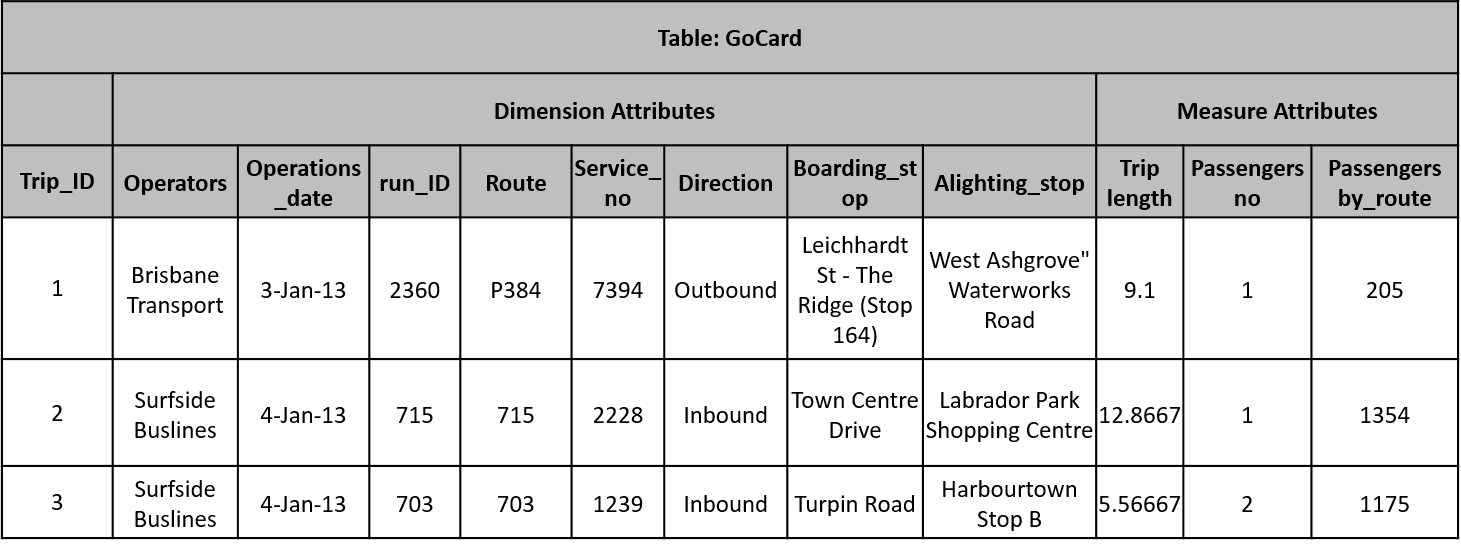
\includegraphics[width=\textwidth]{gocard_schemaandsample.png}
    \caption{Snippet from the GoCard relational database schema with a representative sample. Each row represents one trip with a bus, a ferry or a train with 12 dimensions describing the details of that trip. 
		%
		The database's dimensions are classified into two: dimension attributes and measure attributes, in order to generate meaningful 2-dimensional visualizations, e.g., bar charts.
		}
    \label{fig:gocard_schemaandsample}
\end{figure}
%
%
%
%
%\blue{introduce GoCard data and example.}

The following example illustrates the need for an automatic visualizations technique to identify interesting visualizations from a real, large and structured database called GoCard \footnote{All implementations and data are available online at http://}, which represents trips details of the public transportation system of the Brisbane city in Australia.
%
Figure \ref{fig:gocard_schemaandsample} shows a snippet of the GoCard database schema and a small sample from the database out of the 4.4 million tuples.
%
Each tuple is a record that represents a trip using either a bus, a ferry or a train, with 12 dimensions describing that trip with more details.
%
%
%
\begin{table}[t]
\centering
\caption{Results of query $Q_1$ and $Q_r$: Average trips length in minutes by boarding stop of the view $Q_1$ and the reference view $Q_r$ result into high utility value, i.e., high interestingness. }{
%\begin{center}
\begin{tabular}{|c|c|c|} \hline
& \multicolumn{2}{|c|}{\textbf{Trip Length (min)}}  \\ \hline
\textbf{Boarding Stop} & $Q_1$ & $Q_r$ \\ \hline
	Macarthur Ave : Northshore Hamilton & 74.85 &  34.12\\ \hline
Apollo Ferry Terminal & 70.27 & 26.79\\ \hline
Bretts Wharf Ferry Terminal & 67.01 & 26.24 \\ \hline
Griffith University station  & 61.83 & 11.40\\ \hline
Bulimba Ferry Terminal  & 60.13 & 14.81\\ \hline
%King George Square Station 1A  & 929.3499756 \\ \hline
\end{tabular}}
%\end{center}
\label{tab:q1_result}
\end{table}
%
%
%
%
%
\begin{example}
\label{ex:gocard}
%
Consider a transportation analytic team that is undertaking a study for a particular alighting stop: \emph{University of Queensland} (UQ).
%
This stop has received a lot of passengers’ complaints due to poor performance, hence, it is being investigated by the team.
%
Suppose that the team uses the GoCard database to generate 2-dimensional visualizations (e.g., bar charts) which summarize all recorded trips using different dimensions, then search for the ones that appear to explain the increase in received complaints. 
%
To accomplish that, an analyst would begin by using a program's GUI or a custom 
query language to execute the equivalent of the following SQL query and pull all data from the database for the alighting stop UQ:
%
\begin{center}
\texttt{$Q$ = SELECT * FROM GoCard \\ WHERE alighting stop ="University of Queensland";}
\end{center}
%
Next, the analyst would use an interactive GUI interface to generate all possible visualizations of the query result.
%
%
%containing metrics such as trip length and daily passengers for each route. 
%
%Also, it has a large set of dimension attributes containing information such as operators, service number, operations date, day, direction, boarding stop, alighting stop, etc, as shown earlier in Table \ref{tab:gocard_database}.
%
%Given the large size of the database (millions of records), an analyst will overwhelmingly 
%use a collection of visualization programs to gather insights into the behavior of the alighting stop UQ.
%
%In a typical analysis workflow, 
%
%
For instance, the analyst may visualize average trip length grouped by route, total daily passengers grouped by direction, maximum trip length by boarding stop, and so on. 
%
Hence, the analyst would manually study all these visualizations to find interesting insight or visualizations that might explain the  reason behind the increase of complaints.
%
Indeed, exploring and studying all visualizations is challenging especially for high dimensional datasets.  %impossible.
%
Hence, an automatic visualization recommendation technique should show the analyst the most interesting visualization based on the alighting stop UQ.
%
%Under the hood, these visualization operations are essentially queries to the underlying database and subsequent graphing of the results. 
%

Consider the visualization for the average trip length by boarding stop: it is generated by running an operation equivalent to the following SQL query:
%
\begin{center} 
\texttt{ $Q_1$ = SELECT boarding stop, AVG(trip length)  FROM GoCard 
\\ WHERE alighting stop ="University of Queensland"  GROUP BY boarding stop; } 
\end{center}
%
Table \ref{tab:q1_result} shows the result of running $Q_1$.
%
Consequently, the 2-dimensional bar chart visualization of $Q_1$ (Figure \ref{fig:q1_vis}) happened to be the most interesting visualization.
%
The reason is, when $Q_1$'s result is compared with entire data, it depicts long average trip length in some boarding stops which travels towards UQ that are significantly different from the equivalent average of the trip lengths (equals 17.6 minutes) in the entire dataset.
%
Specifically, $Q_1$'s result is compared against the following reference query $Q_r$:
%
\begin{center} 
\texttt{ $Q_r$ = SELECT boarding stop, AVG(trip length)  FROM GoCard 
\\  GROUP BY boarding stop; } 
\end{center}
%
\qed
\end{example}
%
%
%
\begin{figure}[t] 
	\centering
	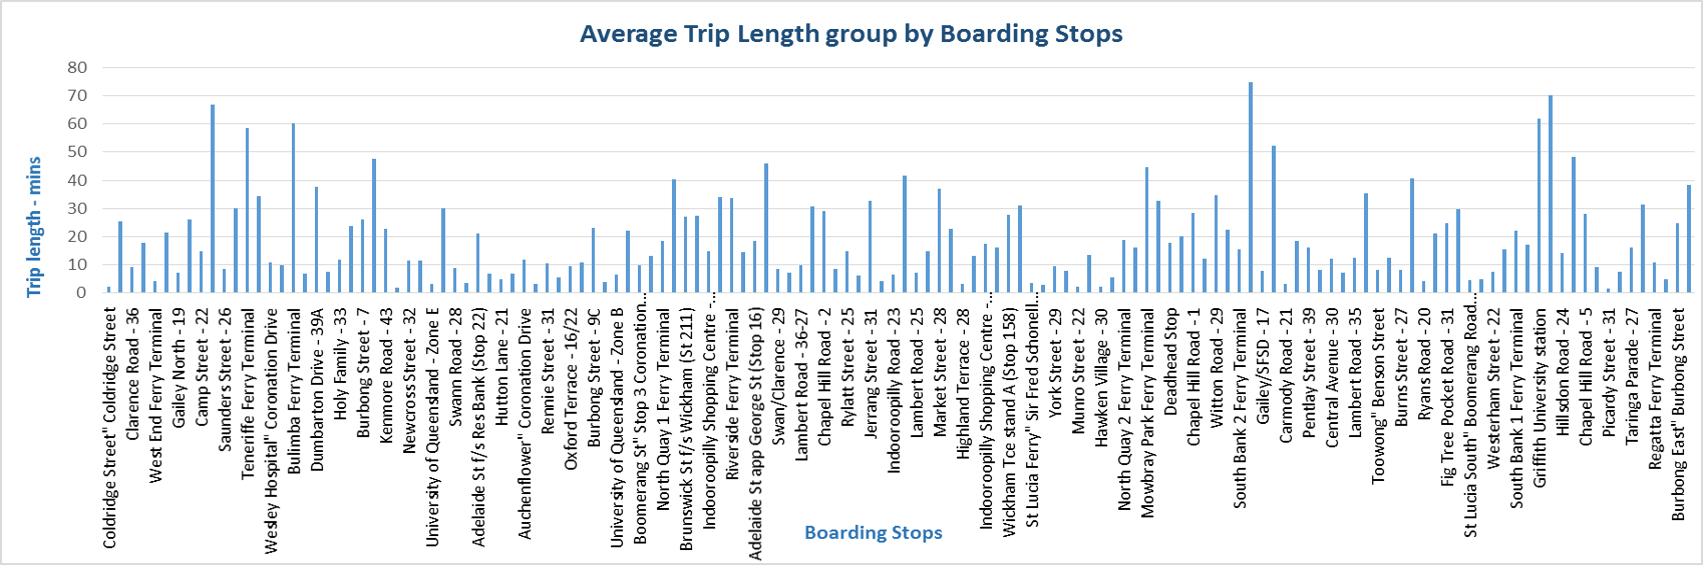
\includegraphics[width=\textwidth]{example.png}
 	\caption{2-Dimensional bar chart visualization generated by query $Q_1$. The x-axis represents the boarding stop, while the y-axis represents the average trip lengths in minutes, towards University of Queensland” stop.}
	\label{fig:q1_vis}
\end{figure}
%
%
%
%
%
%
%
Example \ref{ex:gocard} above suggests that visualizations that portray trend deviations from a reference are potentially remarkable and of high interest.
%

Here, the average trip length grouped by boarding stops (Figure \ref{fig:q1_vis}) is considered as the top interesting visualization, among other visualizations such as total daily passengers grouped by direction, maximum trip length grouped by boarding stop, and so on.
%
The reason is, it depicts long average trip length in some boarding stops which travels towards UQ that are significantly different from the equivalent average of the trip lengths (equals 17.6 minutes) in the entire dataset. 
%
As listed in Table \ref{tab:q1_result}, ferry terminals scored longer trips to UQ than bus stops because ferries often take longer waiting times among stops than buses.
%
%
%
%
%\blue{
\eat{
SeeDB is a data querying and visualization tool that allows analysts to 
manually generate their own visualizations, 
or get data-driven recommendations on demand based on the deviation in data.
%
Specifically, it implements a deviation-based utility metric to identify the most interesting visualizations 
from a large set of potential visualizations. 
%
Then, it posits that a visualization is potentially \emph{interesting} if it 
shows a trend in the subset of data selected by the analyst (i.e., metrics about UQ) 
that deviates from the equivalent trend in the overall dataset. 
%
%}
In our Example \ref{ex:gocard}, the average trip lengths grouped by boarding stops (Figure \ref{fig:gocard_data}) is 
considered as the top interesting visualization produced by SeeDB.
%

However, some bus stops obtained long trips according to the geographical location or the distance such as \emph{Griffith University station}. 
%
%\blue{Abdullah: It is diffcult to know that this view is interesting, so we propose...}
%
%\blue{Add Gap here. Then add list of contribution, then roadmap. Then move to preliminaries and background.}
%\rply{I think we will make the roadmap tomorrow together }
%
}
%
%
%
%
%
%


We summarize our contributions as follows:
%
\begin{itemize}
	\item Proposing a new problem which address the limitation of current visualizations recommendation tools. Particularly, we include budget constraints to automatically
	 recommend top-$K$ interesting visualizations according to an input query within the specified budget.
	 \item Designing an efficient framework called \emph{Realtime Scoring Engine} ($RtSEngine$)
 that limits the exploration of visualizations by assessing priorities of the 
 recommended views according to their deviation utilities and costs.
	\item Proposing efficient algorithms which utilize statistical features of the views such as number 
	of distinct values, selectivity ratios, and data distribution, to early prioritize the views.
	\item Proposing efficient algorithms to approximate the retrieval and computations costs of the generated 
	visualizations and evaluate their estimated costs against their deviation 
	utilities to recommend high accuracy views in the specified budgets.  
	\item Conducting extensive experiments that demonstrate the efficiency and effectiveness of our proposed algorithms on real and synthetic data set.
\end{itemize}
%
This paper is organized as follows: Section \ref{sec:related} describes related works on query visualization. 
%
Then, Section \ref{sec:prelim} provides preliminary details on recommendation of query visualizations and present our problem statement. 
%
Then, we present our framework $RtSEngine$ in Section \ref{sec:method} that contains two main modules: Priority Evaluator and Cost Estimator, which recommend a set of visualizations efficiently within the specified constraints. 
%
Section \ref{sec:expr} shows experiment results for our proposed algorithms on two real datasets. 
%
\section{Background and Preliminaries}
%\section{Preliminaries}
\label{sec:prelim}
%
%\blue{Why mention SeeDB? is this model of visualization exclusive to SeeDB? I think it is general and SeeDB does not own it.}
%\rply{yes it's but we use SeeDB in our experiments as engine, that's why }
%
In this section, we present background details on visualizations in the context of structural databases.
%
We start by explaining how a visualization (or a view) is constructed by an SQL query. 
%
Then, we define our scope of visualizations that our framework is focused on, and how to measure the interestingness of a visualization based on a model proposed by \cite{DBLP:journals/pvldb/VartakMPP14} and another model that we believe is important.
%
Then, we formally present our problem statement.
%

A visualization $V_i$ is constructed by an SQL select-project-join query with a group-by clause over a database $D$.
% 
The dimensions in a database table are classified into two sets: dimension attributes set $A=\{a_1, a_2, ...\}$, and measure attributes set $M=\{m_1, m_2, ... \}$. While the set $F=\{f_1, f_2, ... \}$ contains all aggregation functions.
%
Hence, each visualization $V_i$ is represented as a triple $(a, m, f)$, where $a$ is an attribute applied to the aggregation function $f$ on a measure attribute $m$.
% 

We limit our scope of visualizations on the basic compnents of most 2-dimensional visualization systems: bar charts, line charts and scatter plots, as they satisfy a wide range of applications requirements \cite{Jugel:2016:VAV:2884416.2884424}. 
%

As an example, $V_i(D)$ visualizes the results of grouping the data in $D$ by $a$, and then 
aggregating the $m$ values using $f$. 
%
This view is called the \emph{reference view}.
%
Consequently, $V_i(DQ)$ represents a similar visualization applied to the result set denoted as $DQ$ for a given user query $Q$, and is called the \emph{target view}.
%
An example of a target view is shown in Figure \ref{fig:q1_vis} where $a$ is the boarding stops, $m$ is the trip length, and $f$ is the average aggregation function.
%

Any combination of $(a, m, f)$ represents a view. Accordingly, we can define the total number of possible views as follows:
%The \emph{view space size} $(SP)$ is defined as the total number of views generated.
%
%Specifically:
%
\begin{equation}
\text{View Space} (SP) = 2 \times |A| \times |M| \times|F|
\label{eq:viewspace}
\end{equation}
%
%
%
\eat{
\begin{figure}[t] 
	\centering
	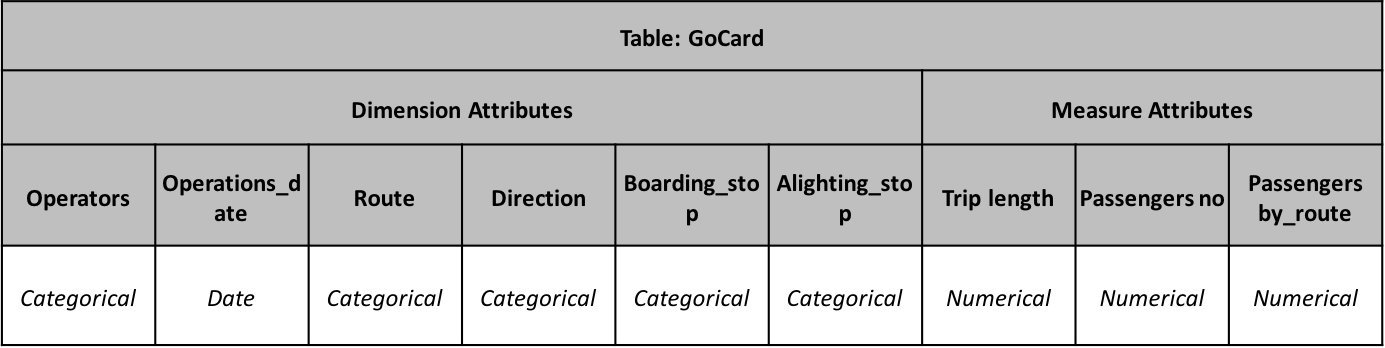
\includegraphics[width=\textwidth]{gocard_sp.png}
 	\caption{GoCard database's dimensions are classified into two: dimension attributes or measure attributes, in order to generate meaningful 2-dimensional visualization such as bar charts.}
	\label{fig:gocard_sp}
\end{figure}
%
}
%
\begin{example}
  \label{ex:gocard_sp}
 %
Using the GoCard database in Example \ref{ex:gocard}, the dimensions within that database can be classified as follows: the set of dimension attributes is $A$ = \{Operators, Operation date, Route, Boarding stop, Alighting stop, Direction\}, while the set of measure attributes is $M$ = \{trip length, passengers by route, passengers no\}, and the set of aggregate functions is $F$ = \{\texttt{count , sum , avg, max, min}\}, as shown in Figure \ref{fig:gocard_schemaandsample}.
%
Therefore, the view space of GoCard database is: $ 2 \times 6 \times 3 \times 5 = 180 $.
%
\end{example}
%
%
Though, in the context of Big Data, $SP$ is potentially a very large number. 
%
Hence, there is a need to automatically rank all these $SP$ views so that exploring them become efficient and practical.
%
To do that, each view is associated with a \emph{utility} value.
%
%
The utility of a visualization is measured as its deviation from a reference dataset $D_R$.
%
For instance, visualizations that show different trends in the query dataset (i.e. $DQ$ ) compared to a reference dataset $D_R$ are supposed to have high utility.
%
The reference dataset $D_R$ may be defined as the entire underlying dataset $D$, the complement of $DQ (D - DQ)$ 
or data selected by any arbitrary query $Q'(DQ')$.
%

Given an aggregate view $V_i$ and a probability distribution for a target view $P(V_i(DQ))$ and a reference view $P(V_i(D_R))$, the utility of $V_i$ is the distance between these two normalized probability distributions.
% 
The higher the distance between the two distributions, the more likely the visualization is to be interesting and therefore higher utility value.
%
%The utility of $U(V_i)$ is defined as the distance
%between the two normalized probability distributions of the target and comparison views.
%
Formally:
%
\begin{equation}
\label{eq:utility}
U(V_i) = S( P(V_i(DQ)), P(V_i(D)) )
\end{equation}
%
\blue{Where $S$ is a distance function (e.g., Euclidean distance, Earth Movers distance, etc). or correlation as reviewer 5 wanted.}
%\blue{it can be any type of distance function, e.g., Euclidean distance, $L_p$-norm, earth movers, etc.}
%\rply{OK}
%
Hence, the problem of visualizations recommendation is as follows \cite{DBLP:journals/pvldb/VartakMPP14}:
%
\begin{definition}
Given a user-specified query $Q$ on a database $D$, a reference dataset $D_R$, a utility function $U()$, and a positive integer $K$. 
%
Find Top-$K$ aggregate views $V_1, V_2, ..., V_K$ that have the highest utilities among all views while minimizing total computation time.
%
\end{definition}
%

Now, we are in place to present our problem statement for visualization recommendations.
%
\subsection{Problem Statement}
\label{sec:problem_statement}
%
Our proposed problem statement for visualization recommendations incorporates two limits (i.e., input parameters) to overcome the limitation of exploring all views.
%
%
\begin{definition}
\label{def:problem}
%
Given a user-specified query $Q$ on a database $D$, a reference dataset $D_R$,  a utility function $U()$, a positive integer $K$, an execution time limit $tl$ or a views number limit $R$ where $K \leq R \leq SP$.
%
Find Top-$K$ aggregate views $V \equiv (a, m, f )$ which have maximum utilities $U(V)$ among all possible views in the 
specified limits $R$ or $tl$ while maximizing the accuracy among all Top-$K$ views chosen from all $SP$ views.
%
\end{definition}
%
The limits $tl$ and $R$ in Def. \ref{def:problem} are added explicitly to overcome the limitation of exploring all views.
%
The former is a time budget that any algorithm should not exceed, while the latter is an upper bound on the number of views to be explored.
%
For instance, $tl$ can be set to zero, and $R = SP$. That is, no limit on the execution time and no limit on the number of generated views.
%
%\blue{extreme cases for $tl$ and $R$, unlimited time, $R$ equals $SP$.}
%

While those limits can be tuned by any valid value, an algorithm should output the same views as if there were no limits. 
%
This requirement makes the problem non-trivial, hence, we address it by presenting our optimization techniques encapsulated within the $RtSEngine$ framework.
%
%Next, we present our optimization techniques which address this challenge efficiently.
\section{Methodology: $RtSEngine$ Framework}
\label{sec:method}
%
%\blue{how this section is org, 2-3 sentences, later when this whole section is completed.}
%
The goal of $RtSEngine$ is to recommend a set of aggregate views that are considered interesting because of their abnormal deviations.
%
%Also, the recommendation process will be tuned with certain realtime limits, i.e., number of explored views $R$ and execution time $tl$.
% 
To achieve that, $RtSEngine$ utilizes the following key idea: recommend views that are created from grouping high ranked dimension attributes $A'$ within the set $A$.
%
The attributes ranks in $A'$ are computed using our proposed prioritizing techniques discussed later in the following sections.
%
%The suggested aggregate views are created from grouping high ranked dimension attributes which evaluated using our proposed prioritizing techniques presented in section \ref{sec:method}. 
Essentially, those techniques evaluate the priorities of all dimension attributes according to their statistical features gathered from the meta-data, e.g., number of selected values, data distribution, and selectivity.
% 
Then, by reordering all dimension attributes according to their priorities, only a subset of high priority attributes are passed to the execution engine, hence, limiting the number of examined views and execution time.  

Conceptually, $RtSEngine$ is designed as a recommendation plug-in that can be applied to any visualization engine, e.g., Tableau and Spotfire.
%
However, in this work, we built $RtSEngine$ as a standalone end-to-end system on top of SeeDB which allows users to pose arbitrary queries over data and obtain recommended visualizations.
%
%\mas{again, cost estimation is not a contribution, it is just a parameter. It is pretty much the same as estimating number of distinct values}
$RtSEngine$ is comprised of two main modules (See Figure \ref{fig:arch}):
%
\begin{figure}[t]
\centering
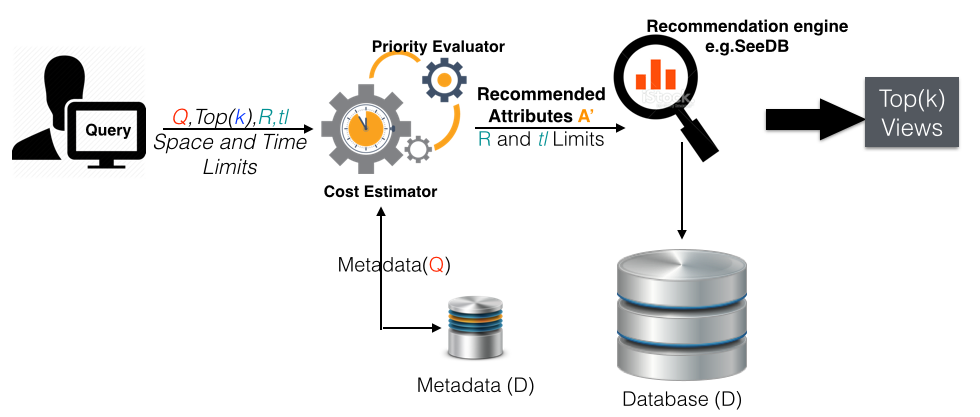
\includegraphics[width=\textwidth]{arch_new.png}
%\subfloat[fig2:Accuracy] {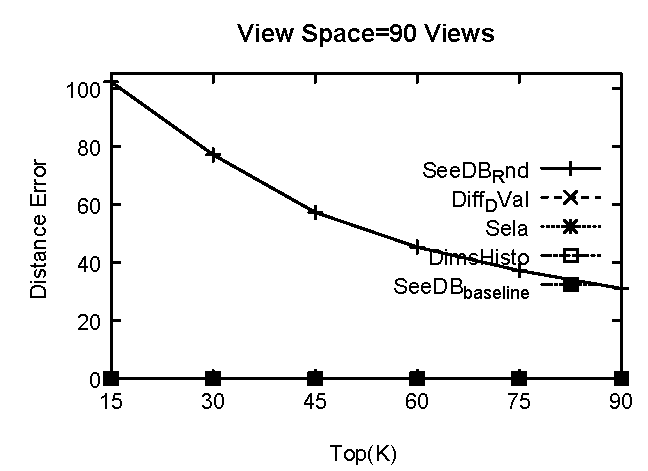
\includegraphics[width=2in]{12.pdf}}
\caption{$RtSEngine$: Real time Evaluation Architecture for Automatic recommendation}
\label{fig:arch}%
\end{figure}
%
\begin{enumerate}
\item \textbf{Priority Evaluator:} An underlying module in front of any recommendation engine. 
%
Used to evaluate the dimension attributes that form visualizations according to a priority function $Pr$ computed using our proposed techniques.
%
\item \textbf{Cost Estimator:} This module is supposed to run in parallel with the Priority Evaluator to estimate the retrieval and computation costs of each visualization using our estimation approaches. 
%
Estimating the visualization costs in real-time improves the efficiency by discounting high costs and low priorities visualizations. 
%
Note that this module is an awareness cost approach which incorporates the estimated costs to assess visualizations based on their priorities and costs.
%
\end{enumerate}
%
We define a notion of benefits $Benefit(V_i)$ of a view $V_i$ as the gains from each view represented as the utility of view $U(V_i)$, compared with the time spent $Cost(V_i)$ to compute the view $V_i$.
%
Formally:
%
\begin{equation}
\label{eq:profit}
Benefit(V_i)= \frac{U(V_i)}{Cost(V_i)}
\end{equation}
%

Cost estimations of visualizations is discussed later on Section \ref{sec:cost_est}.
%
Both modules (Priority Evaluator and Cost Estimator) read information by querying metadata to collect information about dimension attributes, e.g., number of distinct values and cardinality.
%
Next, we describe the two modules in details.
%
%\subsection{Priority Evaluator: Dimension Attributes Prioritizing}%
%\label{sec:priority_evaluator}
%
%\subsection{Cost Estimator: Visualizations Cost Estimation}
%\label{cost_estimator}
%
%\subsection{Priority Evaluator: Dimension Attributes Prioritizing}
%\label{sec:priority_evaluator}
\subsection{Priority Evaluator: Dimension Attributes Prioritizing}
\label{sec:priority_evaluator}
%
%\mas{lots of language problems}
In this section, we discuss the proposed approaches for
prioritizing the dimension attributes in the both results set $DQ$ and reference 
set (e.g. the entire dataset $D$) and suggest a set of visualizations that are likely 
to be interesting and score high deviation utilities in certain realtime limits 
such as maximum number of explored visualizations and execution time.
The proposed approaches are based on our observations about 
the difference between the number of distinct values in the dimension attribute in 
the results set $DQ$ and the entire dataset $D$ affects on the deviation measures. 
In addition, other statistical features may also affect such as data distribution 
and selectivity; such features will be discussed in more detail in the next subsections.
 The following example illustrates this observation and 
describes how our strategies are agnostic for any recommendation system. 
%

%\mas{again, very bad english!}
\begin{example}
\label{ex:priority}
%\end{Exa}
%Consider an airport analytics team that
%is tasked with studying the metrics for all flights departure
%from Origin1, these flights that have poor performance \mas{what does that mean?}. 
Suppose a flights database  keeps flights records which contains two
dimension attributes such as destination airport name and airlines and one
metric is arrival delays. Given the large size of the database
(millions of records) contains 100 airports and 20 airlines
companies, the analyst will study the average delays
visualizations grouped by airports and airlines using a recommendation tool e.g. SeeDB and comparing
these views with a reference set to glean insights about all flights
departure from $Origin1$.
%
These views can be expressed as SQL queries:
\footnotesize
\begin{itemize}
\item $V_1$: select AVG (arrival delays), airport from flights where origin='Origin1'  group by airport;
\item $V_2$: select AVG (arrival delays), airlines from flights where origin='Origin1' group by airlines;
\end{itemize}
%\normalsize
%
\qed
\end{example}
%
For instance, both visualizations $V_1$ and $V_2$ in Example \ref{ex:priority} have the same number of distinct values: 10 
destinations airports and 10 airlines operators.
%
Eventually, aggregate views $V_1$ and $V_2$ will be compared to the corresponding reference views (i.e., the entire dataset $D$) according to a metric.
%
In \cite{DBLP:journals/pvldb/VartakMPP14} for instance, it uses a deviation-based metric that 
calculates the distance between the normalized distributions between the target and reference views. 
%
In our Example \ref{ex:priority}, the average arrival delays of 10 destinations airports in view $V_1$ are evaluated against the average arrival delays of 100 destinations airports 
in the entire dataset $D$.
%
Similarly, the average arrival delays of the 10 airlines operators in view $V_2$ are compared against the average arrival delays of the all 20 airlines operators in the entire dataset $D$.
 %to obtain the distance of $V_1$ \mas{distance from what?}. 
 %To compute the utility distance \mas{utility, distance, or deviation?} there is 
Thus, only 10 distinct values in view $V_1$ will be compared with equivalent values in the reference view, while the remaining 90 distinct values would have no equivalent values in the target view.
%
As a result, those remaining 90 distinct values will be compared with zeros.
%and the remaining 90 distinct values will be compared with 0s, 
% 

Furthermore, in view $V_2$ there are only 10 airlines operators that would be compared with zeros.
% 
This illustration arises a question about the impact of the difference in distinct values of views and their data deviations according to distance-based metrics.
%
% however, when the query returns a smaller number of airports; this means that the 
 %computed distance will be higher \mas{hight than what? why?} than the 
 %distance of $V_1$ \mas{I have no idea what does that sentence mean?}. 
 %Correspondingly, the number of distinct values in the airlines dimension affects on the 
 %utility distance of $V_2$ \mas{??!!}.
%
%\mas{to formalize what? as one of the reviewers mentioned, that example did not lead anywhere}
%\mas{why do you need the term $Dval(v_i(DQ))$ then call it $N$? }
Formally, $Dval(V_i(DQ))$ is defined as the number of distinct values in a target view $V_i$.
%
Consequently, $Dval(V_i(D))$ is the number of distinct values in the corresponding reference view $V_i$.
%
In Example \ref{ex:priority}, $Dval(V_1 (DQ)) = 10$ and $Dval(V_1 (D)) = 100$.
%
As mentioned previously, the deviation of each visualization is captured by a distance based metric that computes the distance between two probability distributions of views.
%
That is, the deviation of a visualization $V_i$ is its utility defined in Eq. \ref{eq:utility}: $U(V_i) = S( P(V_i(DQ)), P(V_i(D)) )$.
%
%i.e., $U(V_i) = S( P[V_{i}Q (x_i)], P[V_{i}D (y_i)])$ 
%where $V_{i}Q (x_i)$ and $V_{i}D (y_i)$ 
%
The distance metric $S()$ is a distance function such as Euclidean, Earth-Mover distance, ... , etc.


We discuss the influence of the difference in distinct values on computing the view utility 
$U(V_i)$ using Euclidean distance (although our experiments are using Earth Movers distance function as the default deviation measure).
  %the number of distinct values of the view $V_i(DQ)$ and $V_i(D)$ \mas{number of distinct values is defined for a column not a view!},
%where $0 < N \leq N'$, the utility of $V_i$ is the distance between 
%the two probability distributions \mas{big notation mess starts here! why defining something, then use =, then use another notation?! Besides couldn't find that $V_{i}Q$ in the table of symbols} $V_i(DQ) = V_{i}Q$ and $V_i(D) = V_{i}D$,
%i.e., 
%$U(V_i) = S( P[V_{i}Q (x_i)], P[V_{i}D (y_i)])$ 
%where $V_{i}Q (x_i)$ and $V_{i}D (y_i)$ are the values by any aggregate function $F$ of
%measure $M$ over group by attribute $A$.
%
%The distance $S$ is distance measure between the two views;
%this distance measure could be Euclidean, Earth-Mover
%distance, or others. 
%
%However, in this example \mas{which example?} we discuss the
%influence of number of distinct values on the view utility
%using Euclidean distance and also consider the Earth-Mover
%distance \mas{is EMD actually discussed?}.
 As shown in Eq. \ref{eq:ec_d}, $L_2$-norm distance evaluates all aggregated values (points) in both views $V_i(DQ)$ and $V_i(D)$ to find the utility $U(V_i)$. 
%
Hence, $V_1$'s utility in Example \ref{ex:priority} is obtained by computing the $L_2$-norm distance between the average arrival delays (values) of destination airports (points) in $V_1(DQ)$ and all airports in $V_1(D)$ the entire dataset.
% \mas{is it V or D? }
%
Formally:
%
\begin{equation}
\label{eq:ec_d}
U(V_i) = \sqrt{ \sum^{n}_{j=1}{(V_{i}D(y_j) - V_{i}DQ(x_j))^2}}
\end{equation}
%
where $n > 0$ is the maximum number of points among $V_{i}D$ and $V_{i}DQ$.
%
Since the compared views (i.e. target and reference view) may contain different number of distinct values, we denote $n'$ as the number of records in $V_i(DQ)$ 
and $n''$ as the number of records in $V_i(D)$.
%
Hence, we can rewrite the utility equation of view $V_i$ as follows:
%
\begin{equation}
\label{eq:ec_d2}
U(V_i) = \sqrt{ \sum^{n'}_{j=1}{(V_{i}D(y_j) - V_{i}DQ(x_j))^2} + \sum_{j=n'+1}^{n''}{(V_{i}D(y_j) - 0)^2} }
\end{equation}
%
where $n' < n''$, and $n = n' + n''$.
%
Because there are only $n'$ values in the target view $V_{i}DQ$, then all subsequent points in the reference 
view $V_{i}D$, i.e., $n'' - n'$ values, would be compared with zeros.
%
The higher the difference between distinct values in corresponding views forces much remaining values 
to be compared with zeros and increases the distance among views.
%
In Example \ref{ex:priority}, the number of records $n'$ of both target views 
$V_1(DQ)$ and $V_2(DQ)$ equals 10. 
%
However, the number of records in the reference views, i.e., $n''$ are $V_1(D) = 100$ and $V_2(D) = 20$.  
%
$V_1$ is expected to show higher distance (deviation) than $V_2$ when computing 
$L_2$ norm distance because 90 airports would be evaluated to zeros in $V_1$ but there are only 10 airlines operators with zero values in view 
$V_2$. 
%
Since, every view is an aggregate group by query over a dimension attribute as described earlier, then, the number of records in 
each view equals the number of distinct values in the grouped dimension attribute.
%

Such observations can be utilized to early asses these (visualizations) views before executing the underlying queries to avoid computational costs (i.e., retrieval and deviation measure costs) by evaluating dimension attributes that contribute in creating visualizations.
%
Furthermore, evaluating dimension attributes can also be done using other statistical properties such as selectivity and data distribution.
%

Further discussion of utilizing these features in our proposed approaches is presented in the next sections.
% about the difference between 
%the number of distinct values in the dimension attribute in the results set and the entire dataset \mas{yes there is a "difference", but what is the observation?!!!}. 
%%
%This means, how much change of the distinct values in each dimension 
%attribute before and after the user query. Similarly, the bigger a view size 
%(i.e has many distinct values) that produced from attribute $A$, has a lower utility \mas{why?} distance 
%than the smaller view created over the same dimension attribute and the same measure 
%compared with the entire dataset because the number of distinct points that compared 
%with zero is less than those in the smaller view \mas{and why would that lead to lower utility?!!}.
%

\subsubsection{Ranking Dimension Attributes based on Distinct Values} 
%
\begin{algorithm}[t]                      
\caption{$Diff_DVal$}          
\label{alg:diff_dval}                                         
\KwIn{ Attributes $A(a_1, a_2, ..., a_n)$ , Query $Q$, Views limit $R$ }
\KwOut{Set $\mathcal{H}$: Highest priorities of dimension attributes}
$\mathcal{C} = \phi$ Set of all dimension attributes priorities \;
\For{ $i = 1 $ \textbf{to} $n$ }{
	    $Dval D(a_i) \gets$ number of distinct values of $a_i$ in $D$   \;
	    $Dval DQ(a_i) \gets$ number of distinct values of $a_i$ in $DQ$ \;
	    $Pr(a_i) = |Dval D(a_i) - Dval DQ(a_i) |$\;
	    $\mathcal{C} \gets Pr(a_i)$\;
	}
	Sort $\mathcal{C}$\;
	$G= |\frac{R}{M \times F}|$ \text{Calculate the required dimension number}\;
	%\COMMENT Find high utilities dimension attributes $S\{\}$
	\For{$i = 1 $ \textbf{to} $G$}{
		$\mathcal{H} \gets \mathcal{C}.get(i)$\;
		}
		\Return{ $\mathcal{H}$}\;
\end{algorithm}
%
%\subsubsection{Ranking dimension attributes based on distinct values}
%
%\mas{an algorithm name cannot be symbols! use a proper name!}
%\mas{How is it related to Jaccard index?}
%
Scoring dimensions based on difference of distinct values is the first class of prioritizing algorithms.
%
This approach is referred to as $Diff_DVal$, and it is based on the basic observation 
about the number of distinct values of the dimension attributes in 
the results set $DQ$ and the entire database $D$. 
%
The $Diff_DVal$ algorithm scores the dimension attributes according
to the difference between the normalized distinct values of attributes in the 
result set $DQ$ and the entire database $D$. 
%
Algorithm \ref{alg:diff_dval} inputs a query $Q$, a set
of dimension attributes $A$, maximum views limit $R$, and/or execution time limit $tl$. 
%
Then $Diff_DVal$ obtains the number
of distinct values for all dimension attributes in both results sets $DQ$ and reference dataset $D$ by posing underlying queries to select the count of distinct values. 
%
After getting the number of distinct values, $Diff_DVal$ computes the priority of each dimension attribute 
%\mas{make it clear that you are converting the problem from views to dimension attributes} 
as the difference between each normalized values. 
%
Then, $Diff_DVal$ sorts all dimension attributes based on their priorities.
%
Based on Eq. \ref{eq:viewspace}, $Diff_DVal$ computes the required number of dimension attributes $G$ that creates the limit number of views $R$, then it returns the set $\mathcal{H}$  of size $G$ that contains a group of high priorities attributes.
% Since the visualization space size is defined previously as the total number of all possible visualizations which equals the product of number of dimension attributes $A$, number of measure attributes $M$, and number of aggregate functions $F$,  algorithm $Diff_DVal$  computes the required number of dimension attributes $G$ that creates the limit number of views $R$ then outputs a set of high priorities $Pr$ attributes of size $G$.

In case there is an execution time limit $tl$, $Diff_DVal$ returns an ordered set of all dimension attributes based on their priorities, and then it passes the time limit $tl$ to the recommendation visualization engine to limit the executions.
%\mas{but it does not consider the execution time, in the presence of time limit?}
 


%\subsubsection{Scoring dimension attributes based on Selectivity}
\subsubsection{Scoring Dimension Attributes based on Selectivity}
\label{sec:sela}
%
\begin{algorithm}[t]                      
\caption{$Sela$}          
\label{alg:sela}                           
%\begin{algorithmic} [1]                  
\KwIn{ Attributes $A(a_1, a_2, ..., a_n)$ , Query $Q$, Views limit $R$ }
\KwOut{Set $\mathcal{H}$: Highest priorities of dimension attributes}
$\mathcal{C} = \phi$ Set of all dimension attributes priorities \;
\For{ $i = 1 $ \textbf{to} $n$ }{
	    $Dval D(a_i) \gets$ number of distinct values of $a_i$ in $D$   \;
	    $Dval DQ(a_i) \gets$ number of distinct values of $a_i$ in $DQ$ \;
	     $Pr(a_i) = Dval DQ(a_i) * Sel^{DQ}_{a_i} + (\frac{Dval DQ(a_i)}{Dval D(a_i)}) * Sel^{D}_{a_i}$\;	     
			$\mathcal{C} \gets Pr(a_i)$\;
	}
	 Sort $\mathcal{C}$\;
	$G= |\frac{R}{M \times F}|$ \text{Calculate the required dimension number}\;
	%\COMMENT Find high utilities dimension attributes $S\{\}$
	\For{$i = 1 $ \textbf{to} $G$}{
		$\mathcal{H} \gets \mathcal{C}.get(i)$\;
		}
		\Return{ $\mathcal{H}$}\;
\end{algorithm}
%
In this section, we discuss another variation of scoring the dimension attributes by capturing the data distribution in 
terms of query size and selectivity.
%
Selectivity estimation is at the heart of several important database tasks. 
%
It is essential in the accurate estimation of query costs, and allows a query optimizer to characterize good query execution plans from unnecessary ones. 
%
It is also important in data reduction techniques such as in computing approximated answers to queries \cite{DBLP:journals/debu/BarbaraDFHHIJJNPRS97,DBLP:conf/pods/GilbertKMS01}. 
%
Databases have relied on selectivity estimation methods to generate fast estimates for result sizes \cite{DBLP:conf/sigmod/ChaudhuriMN98,DBLP:conf/pods/CharikarCMN00,DBLP:journals/csur/ManninoCS88,DBLP:conf/sigmod/Piatetsky-ShapiroC84}.
%
%This is typically used in cost-based query optimizations, online aggregations, assessing the uniqueness of data,and statistical studies.
%

The selectivity ratio \cite{lahdenmaki2005relational} is defined as follows:
\begin{definition}
The degree to which one value can be differentiated within a wider group of similar values.
\end{definition}
%
The selectivity ratio also known as the number of distinct unique 
values in a column divided by its cardinality \cite{DBLP:conf/sigmod/KeyHPA12}.
%
Formally, the selectivity ratio of attribute $a_i$ is:
%
\begin{equation}
\label{eq:selec_ratio}
Sel_{a_i}^{B} = \frac{ \text{Number of distinct values of $a_i$ in $B$} }{ \text{Cardinality of $a_i$ in $B$} }
\end{equation}
%
where $B$ is either the result set $DQ$ or the reference dataset $D$, and $0 < Sel^{B}_{a_i}  \leq 1$.

%
For the flight database in Example \ref{ex:priority}, both the result set $DQ$ and the reference set $D$ have a fixed number of records, which reveals that the selectivity ratio of the airlines column is usually low because we cannot do much filtering with just the 20 values. 
%
In contrast, the selectivity ratio of the airports column is high since it has a lot of unique values.
%
Our proposed approach $Sela$ utilizes the number of distinct values in the dimensions attributes and incorporates the query size to identify priorities of these dimensions by calculating a %\mas{is it scoring or utility or priority?! isn't it already defined much earlier?}
priority function $Pr()$ for each dimension attribute. 
%
Then $Sela$ reorders the dimension attributes based on the priority. %to prune \mas{prune?} low utility dimension attributes from the data space \mas{what is the data space?}. 

%
%To discuss the approaches, we collect metadata information for each dimension 
%attribute $a_i$ in $D$, such as, the selectivity ratio $SelD(a_i)$ of attribute $a_i$ is a measure 
%of how much variation of data in attribute $a_i$ as:
%\[
%SelD(a_i) = \frac{number\_of\_distinct\_values}{number\_of\_records\_of\_D}
%\]
%\mas{that Dval thing was defined in terms of views before, is it now defined on attribute?}
%Where the selectivity ratio is a value between [0-1], $0 < SelD (a_i)  \leq 1$, and the number of distinct values ($Dval D(a_i)$) of the attribute $a_i$, which considered as a measure for the number of data points that would be competed in attribute $a_i$ as:
%\[
%Dval D(a_i) = number\_of\_distinct\_values\_in\_attribute\ a_i\_D
%\]

Using selectivity ratio and the number of distinct values for assessing 
visualizations in $D$ and $DQ$ gives closer insights 
%\mas{how?} 
about the data characteristics such as the size (number of records) of aggregated views generated from 
group by attributes and the uniqueness degree of data in each dimension attribute.
%\mas{which characteristics?} 
%as the change in the size of the views \mas{size of the view - isnt the same as the number of distinct values?} generated by the
 %dimension attributes over a group by aggregate query using any measure attribute and the 
% degree of variation of data in the dimension attributes \mas{what does "the degree of variation of data mean?"}. 
%
%Computing how much the variations in the size of the 
%dimension attributes in datasets $D$ and $DQ$. 
%
%
Again, in the flights database Example \ref{ex:priority}, $DQ$ have 10 distinct airports out of 100 airports in the airports column.
%
This means any visualization constructed by grouping airports column in 
result set $DQ$ contains only 10 aggregated records. 
%
Hence, using the query size assists on quantifying how many records would be aggregated in each view 
that formed from grouping a dimension attribute. 
%
However, capturing the change of both number in distinct values and the number of aggregated records in each dimension attribute in result set $DQ$ and reference set $D$ is essential to identify visualizations that produce high deviations among all possible visualizations.
%
Thus, we modified the priority function $Pr()$ in $Sela$ to consider the number of records in each dimension attribute $a_i$ and its selectivity ratio. Formally:
%
\begin{equation}
\label{eq:prio_sela}
Pr(a_i) = Dval DQ(a_i) * Sel^{DQ}_{a_i} + (\frac{Dval DQ(a_i)}{Dval D(a_i)}) * Sel^{D}_{a_i}
\end{equation}
%
The attribute priority $Pr(a_i)$ evaluates the number of distinct values for each dimension attribute in result set $DQ$ multiplied by its selectivity ratio.
%
This identifies the distinct values variations and the diversity through each dimension attribute when compared with the number of records. 
%
Furthermore, the same number of distinct values is assessed in the corresponding dimension attribute of the reference set $D$ while considering the number of records.
  
In $Sela$, high priority dimension attributes are assumed to produce aggregate views (i.e., target views) that contain many groups (i.e., points) which are aggregated from records in the result set $DQ$. 
%
Also, the same high priority dimension attributes are assumed to produce aggregate views (reference views) 
by aggregating larger number of records in reference set $D$. 
%
This has direct effect on the aggregated values and the number of groups in both target and reference views which is expected to score high deviation utilities. 
%
%In contrast, low priority dimension attribute generates aggregate views which compromise smaller number of groups (points) in both datasets. 

Although the $DiffDval$ approach prioritizes dimension attributes (aggregate views) according to the number of distinct values, it is limited since it is incompetent to prioritize dimension attributes (aggregate views) when the number of distinct values remains stable in both result set $DQ$ and reference set $D$.
%
Moreover, $DiffDval$ does not consider the data distribution within the attributes. 
%
To overcome this limitation, $Sela$ utilizes the number of records and the selectivity ratios of dimension attributes in both datasets $DQ$ and $D$.

%\mas{isnt that basically the number of distinct values squared divided by the number of records?! what is the physical meaning of that component? and what does it mean if it is low or high?} 
%and the how much change in the number of distinct values happened in the entire 
%dataset $D$ multiplied by the selectivity ratio of the dimension attribute 
%in result set $D$ \mas{again what is the physical meaning of that component? wouldnt SelD and DvalD cancel each other?}. 
%This combines the disparity \mas{what is disparity?} in the number of distinct values of the 
%dimension attribute and the deviation of the selectivity ratio in these datasets. 
%
%\mas{besides the meanings of those components, why would that reflect the actual utility? what was the limitation of the first ranking policy, and why does this policy improve upon it?!}

%
The proposed algorithm $Sela$ firstly computes the priority of each dimension attribute based on Eq. \ref{eq:prio_sela}.
%
Then, it sorts the dimension attributes based on the assigned priority to create a set $\mathcal{H}$ of 
the top $G$ dimension attributes.
%
In case of execution time limit $tl$, $Sela$ returns an ordered set of attributes with the highest priorities and passes time limit $tl$ to the recommendation visualization engine to limit the executions. 
%

%\subsubsection{Priortrizing Dimension attributes based on histograms}
\subsubsection{Prioritizing Dimension Attributes based on Histograms}
\label{sec:priority_hist}
%
\begin{algorithm}[t]
\label{alg:prio_hist}
\caption{$DimsHisto$}
\KwIn{ Attributes $A(a_1, a_2, ..., a_n)$ , Query $Q$, Views limit $R$ }
\KwOut{Set $\mathcal{H}$: Highest priorities of dimension attributes}
$\mathcal{C} = \phi$ Set of all dimension attributes priorities \;
\For{ $i = 1 $ \textbf{to} $n$ }{
Compute $HD(a_i)$ and $HDQ(a_i)$\;
$Pr(a_i) = d(HD(a_i), HDQ(a_i))$\;
$\mathcal{C} \gets Pr(a_i)$\;
}
Sort $\mathcal{C}$\;
	$G= |\frac{R}{M \times F}|$ \text{Calculate the required dimension number}\;
	%\COMMENT Find high utilities dimension attributes $S\{\}$
	\For{$i = 1 $ \textbf{to} $G$}{
		$\mathcal{H} \gets \mathcal{C}.get(i)$\;
		}
		\Return{ $\mathcal{H}$}\;
\end{algorithm}
%\mas{since it is basically COUNT, how does it work for ranking other aggregates?}
%\mas{should it be used directly? or try to use the histogram to provide an approximate answer for other aggregates and treat it as the actual answer when measuring distance. There is lots of work on generating such approximate answers starting from: Approximate query answering using histograms, IEEE Data Engineering Bulletins, 1999.}
We proposed $Sela$ and $Diff_DVal$ approaches to automatically recommend views with the highest deviations based on a priority for each dimension attributes in a star schema database $D$.
%
Specifically, the proposed approaches relay on the number of the distinct values and the selectivity ratio of each dimension attribute in the compared datasets (i.e., $DQ$ and $D$) to compute the attributes priorities.
%

However, the limitation
 % \mas{what other limitations?}
of the proposed approaches is using the selectivity ratio 
	%\mas{is it selectivity or number of distinct values or both?} 
to reflect the degree of variations of data in the dimension attributes while ignoring the distribution of data itself. 
%
In addition, it is difficult to prioritize dimensions that have the same distinct values or the same selectivity ratio.
%

%
Hence, we propose the $DimsHisto$ approach which attempts to capture data distribution inside the dimensions attributes by creating frequency histograms and directly measuring the distance among corresponding histograms to evaluate these dimensions attributes.
%
  %then computing
  %how much each dimension attribute in the query result set $DQ$ is deviated from
   %its original version in the entire dataset $D$ by managing \mas{managing?!} the frequency histograms for these 
   %dimensions \mas{and why would a histogram do better?}. 
$DimsHisto$ firstly generates frequency histograms for all dimensions attributes in each dataset. 
%
Then it computes the deviation in each dimension by calculating the normalized distances between each corresponding dimension attribute.
%
For any star schema database $D$, a dimension attribute $a_i \in A =\{a_1, a_2, ... …, a_n\}$ can be represented as two frequency histograms: $H_{D(a_i)}$, and $H_{DQ(a_i)}$.
%
Those two histograms are created by executing the following queries:
\\$H_{D(a_i)}$: Select $count(a_i)$ from D group by $a_i$;\\
$H_{DQ(a_i)}$: Select $count(a_i)$ from DQ group by $a_i$;\\
%
Then, after normalizing these histograms, the priority of each dimension attribute is computed as the distance between these two histograms:
\begin{equation}
\label{eq:pro_hist}
Pr(a_i)= S( H_{D(a_i)}, H_{DQ(a_i)} )
\end{equation}
%
Where $S()$ is a distance metric. 
%
Eventually, the dimension attributes are sorted according to their priorities.
%\mas{isnt the same as measuring the deviation when the aggregate function is count?!}.

%
A constructed histogram $H_{D(a_i)}$ is equivalent to all aggregate views created by aggregating any measure attribute (using aggregate function \emph{Count}) and grouped by the dimension attribute $a_i$ in the dataset $D$.
%
Such a histogram assists in improving the performance of recommendation engines by avoiding the construction and computation of aggregate views along all measure attributes.

%Such that, assists to avoid aggregate views construction and computations for all possible measure attributes which improves the performance of recommendation engines.    
%
%Algo
$DimsHisto$ has to submit $2 \times |A|$ queries to compute the histograms of all dimensions 
and the computations of the distance metric.
%
However, this step can be optimized to only $|A|$ by computing the histograms of all dimensions for the entire database offline.
%
%The proposed algorithm $$ costs $2n$ queries 
%(where $n$ is number of the dimension attributes $A$ 
%\mas{what happened to A?}
%) to compute the histograms of all dimensions 
%and the computations of the distance metric, but the actual number of queries can 
%be declined to $n$ and this optimization can be achieved by computing the histograms of 
%all dimensions for the entire database offline. 
While $DimsHisto$ can use any distance metric to compute the deviation among the views, we suggest to use the same metric to unify the metric of the deviations.
% 

All proposed algorithms $Diff_DVal$, $Sela$ and $DimsHisto$ have the same 
number of queries as the cost of retrieving data.
%
While $DimsHisto$ has additional cost for distance computations, it shows high accuracy for most of the aggregate functions such as Sum, Avg, and Count, because these functions are relative to the data frequencies. 
%
Though, $DimsHisto$ is less descriptive to other aggregate functions such as Min and Max, as they are not amenable for sampling-based optimizations.
%\mas{why?!!!! what is novel about it that makes it better?!} than $Sela$ in our test experiments.
%
\subsection{Cost Estimator: Visualizations Cost Estimation}
\label{sec:cost_est}
%
\begin{algorithm}[t]
\label{alg:viewsest}
\caption{$ViewsEstimate$}
\KwIn{ Attributes $A(a_1, a_2, ..., a_n)$ , Measures $M(m_1, m_2, ..., m_o)$ , Functions $F(f_1, f_2, ..., f_x)$  }
\KwOut{$\mathcal{S}$: set of views estimated costs}
%$\mathcal{C} = \phi$ Set of all dimension attributes priorities \;
\For{ $i = 1 $ \textbf{to} $n$ }{
%$totalCost = 0$\;
\For{ $j = 1$ \textbf{to} $o$ }
{
\For{ $p = 1$ \textbf{to} $x$ }
{
$C(VDQ) = EstCostDQ(a_i, m_j, f_p)$\;
$C(VD) = EstCostD(a_i, m_j, f_p)$\;
$C(d(VDQ,VD))$  Eq.\ref{eq:cost_view_measure}\; 
$Cost = C(VDQ)+ C(VD)+ C(d(VDQ,VD))$ \;
$\mathcal{S}$.add($Cost, (a_i, m_j, f_p)$) \;
}
}
}
\Return{ $\mathcal{S}$}\;
\end{algorithm}
%
%\mas{title is so wrong! First, there is no such thing as cost of a dimension! Second, estimating the cost is trivial and not a contribution.}
%\mas{As i mentioned to you many times, cost estimation is a very mature area. 
%See a paper like: Predicting Query Execution Time: Are Optimizer Cost Models Really Unusable? and ALL its citations..
%So to come up with your new cost estimator, you have to show that none of this well established work is good enough and there is something unique about your queries that requires a new estimator, especially in comparison to the ones using machine learning since they make no specific assumptions about the query execution mode.
%}
The previous approaches rank dimension attributes according to their priorities 
and recommend visualizations while being oblivious to the retrieval and computational costs of those visualizations.
%while considering same retrieval and computational costs for all generated views 
 %\mas{what does that mean?} 
However, visualizations created using different dimension and measures attributes have different retrieval and execution costs 
% \mas{again there is no such thing as cost of dimension!}
according to the query size, type of the aggregate functions, number of groups in each attribute and 
the time used to compute the deviation among all values in the corresponding visualizations.
% 
%Moreover, views produce different utilities when measuring the deviation distance. %\mas{why different utilities affect the cost?}.
%

This urges the need to only generate visualizations with high deviations and avoid the computation costs of the low-deviation ones.
%
Besides differences in deviation utilities among different visualizations, each visualization exhibits different execution and retrieval costs.
%
%Since each view $V=(a,m,f)$ is considered as an aggregate query, each query exhibit different execution and retrieval times (on top of the deviation utilities). 
%
Furthermore, some visualizations may take long computations and retrieval time to only yield small deviation distances. 
%
The trade-off between gaining high utilities of the visualizations and their computations and querying costs is challenging because 
it involves the optimizations of finding high utilities visualizations while considering their costs.
%we define a notion of the benefits $Profit(v)$ of a view $v$ that evaluates the gains from each view as 
%the utility of view $U(v)$ compared with the time spent $Cost(v)$ to compute all execution 
%and computational costs of view $v$.
%\[
%Profit(v)= \frac{U(v)}{Cost(v)}
%\]
%\mas{That should have been brought way earlier, with a general problem definition based on the realtime requirement.}
%Similarly, 
%The profit of a dimension attribute $(a_x)$ is computed as total utilities $U(v)$ 
%of all aggregated views created by  attribute $(a_x)$ along 
%all measures attributes and aggregated functions divided by their costs e.g. 
%\begin{equation}\label{ProftAtt}
%Profit(a_x)= \frac{\sum_{i=1}^M \sum_{j=1}^F U(a_x,m_i,f_j) }{\sum_{i=1}^M \sum_{j=1}^F Cost(a_x,m_i,f_j)}
%\end{equation}

%the $Profit(Top-K)$ is considered as the summation of the \{Top-K\} 
%utilities divided by the time spent for querying and computing in views in the space $SP$
%\[
%Profit(Top-K)= \frac{\sum_{i=1}^K U(v_i)}{\text{All views' costs Space $SP$}}
%\]

%We extend our problem definition to find a set of dimension attributes that produce high deviated
 %views with in the user space limit while considering the space computation costs as following:

%\mas{again again again mixing the problem with solution and no mention of the time constraint! }


%\subsubsection{Problem Definition} \label{PDCost}
%Consider a star schema database $D$ has a set $A =\{a_1,a_2,...,a_n\}$ of dimension attributes 
%and a set $M =\{m_1,m_2,...,m_x\}$ of measures attributes 
%with a view space $SP=A \times M \times F$ where $F$ is a set of aggregate functions, 
%we denote each View $(V_i)=(a,m,f)$  and the result set of the query $Q$ posed over $D$ as $DQ$. 
%The analyst specifies top($K$) deviated views within a view space limit $R$ where $K \leq R$. 
%Find a set $\{A'\}$ of high dimension attributes of $Profit(a_i)$  that 
%creates space $R=A' \times M \times F$ while maximize 
%the accuracy among all top($K$) deviated views  generated using $SP$ and $R$ and minimizing the 
%total computation costs of space $R$. \\

%\mas{long paragraph and it is not clear what is the message? are you making a new contribution in cost estimation?}
The cost estimation step is essential to determine the cost of running and computing the deviations of a visualization to evaluate its costs against 
the utility obtained by measuring the deviation among visualizations. 
%
To improve the performance of recommendation applications, it is vital to discard visualizations that are expected to consume much retrieval and computation time while returning low deviation distances.
%
%which 
% \mas{and why is it needed?}.

The cost estimation modules approximate CPU and I/O costs to combine them into an overall metric that is used for 
comparing alternative plans. 
%
The problem of choosing an appropriate technique to determine CPU and I/O costs requires considerable care. 
%
An early study \cite{Mackert:1986:ROV:16856.16863} identified key roles for accurate cost estimation, such as the physical and statistical properties of data.
%that in addition to the physical and statistical properties of the input data streams 
%and the computation of selectivity, modeling buffer utilization plays a key role in 
%accurate estimation. 
%
%This requires using different buffer pool hit ratios depending on the 
%levels of indexes as well as adjusting buffer utilization by taking into account properties of 
%join methods. 
%
Cost models take into account relevant aspects of physical design, e.g., co-location of data and index pages. 
%
However, the ability to do accurate cost estimation and propagation of statistical information on data remains one of the difficult open issues 
in query optimization \cite{Chaudhuri:1998:OQO:275487.275492}.
%

We determine the cost of a view $Cost(V_i)$ as the sum of the following: 
\begin{itemize}
	\item Cost of running view $V_i(a,m,f)$ on dataset $D$.
	\item Cost of running view  $V_i(a,m,f)$ on dataset $DQ$.
	\item Computation cost of the distance function $S(V_i DQ, V_i D)$.
\end{itemize}
 %the  which represents 
%the cost of calculating the deviation measure among all values of both views $d[(V_i DQ),(V_i D)]$ . 
Formally:
\begin{equation}
\label{eq:cost_view}
Cost(V_i)= C(V_i DQ) + C(V_i D) +  C(S(V_i DQ, V_i D))
\end{equation}
%
%\blue{next sentence is not clear. } The cost of a dimension attribute $(a_x)$ 
%\mas{what does it mean to say cost of a dimension?} 
%is computed as total costs 
%of all aggregated views created by  attribute $(a_x)$ along 
%all measures attributes and aggregated functions.% e.g. 
%\mas{what is view()?}
%\[
%\text{the estimated attribute cost} (a_x)= \sum_{i=1}^M \sum_{j=1}^F view(a_x,m_i,f_j)
%\]

As mentioned previously, the cost of running a view $V_i(a,m,f)$ on a database is affected by various factors. 
%
For instance, access paths and indices that are used to execute the view determine the proper execution plan, which reflects the view execution cost.
%
%t of the view then selection of proper execution plan. 
%Further, memory and disk accesses issues affect on the cost of query like database buffer size 
%and block reading time have essential impact on execution cost of view. 
%
%In addition, the query 
%execution differs on row oriented and column oriented databases which makes the estimation process is 
%challenging. %\mas{so what?} \\

\noindent \textbf{Running Cost of Views $C(V_i DQ)$ and $C(V_i D)$}: 
%
refers to the retrieval cost of the results of both views $V_i DQ$ and $V_i D$ as discussed earlier. 

%\blue{this sentence is not clear. } that it is hardly to obtain the exact execution time however, several work illustrated the different
 %approaches to estimate and approximate the aggregated queries  
 %\cite{Lazaridis:2001:PAA:376284.375718,du1997estimators}
 %and other researches consider the optimizing the execution of aggregated queries  
 %\cite{Hou:1989:PAR:67544.66933,Chaudhuri:1994:IGQ:645920.672834}
 %using different techniques of transformations 
 %\cite{Chaudhuri:1994:IGQ:645920.672834,Afrati909designingan} 
% and developed methods for query rewriting rules of 
% aggregate queries  \cite{Gupta:1995:APD:645921.673150} using group-by operator evaluations. 
%

\noindent \textbf{Computation Cost of $C( S(V_i DQ, V_i D))$}: is considered as the time spent on calculating the distance measure $S()$ for each value in both corresponding views.
%

The number of points that are compared in the corresponding views $V_i DQ$ and $V_i D$ is the maximum number of groups (bins) among these two views, and it is denoted as $n$.
%
Alternatively, it equals the maximum number of distinct values in $V_i DQ$ and $V_i D$ attribute dimension.

%The number of points that are compared in the views is actually the number of groups (bins) $n$ in these views. 
%
Note that the cost of distance measures vary according to their computational complexity. 
%
For example, the Euclidean distance is faster than the Earth Mover $(EMD)$ distance function.
%
This is because $EMD$ has a very high complexity $O(n^3 log n )$  \cite{Jang:2011:LAE:2063576.2063652} while the complexity of the Euclidean distance is $O(n)$.
%

%We denote the size of a view $V_i$ as $Dval(V_i)$, which represent the number of groups in the view.
%
%Alternatively, it equals the number of distinct values in this view's attribute dimension.
%\mas{is N the same as Dval?}
Since the computation cost depends on $n$ and also 
depends on the computational complexity of the distance measure, we propose the following view cost equation:
%\begin{center}
\begin{equation}
\label{eq:cost_view_measure}
C( S(V_i DQ, V_i D)) = O_d( n ) \times d_t
\end{equation}
%\end{center}
Where $O_d$ is the complexity of the distance measure, and $d_t$ is the computation time used to compute a single point.
% the distance between two corresponding points.
 %and  $Dval(V_i DQ)\leq Dval(V_i D)$. \mas{and how to know those values O and d? and more importantly, how is that applied to different distance measures? for instance, EMD is of $O(N^3)$, but now it is linear under this eq!!}

\subsubsection{Retrieval Costs of Visualizations}
\label{sec:ret_cost_view}
%
In our context, the execution cost of views can be obtained using two different methods:
 %
\begin{itemize}
\item \textbf{Actual Cost:} actual costs of the views are obtained by executing all queries to get their exact I/O costs, and calculating the deviation among the corresponding views.
%
\item \textbf{DB Estimates:} reading the estimates of each view directly from the database engine (i.e., query optimizers).
%\item[Computational Estimates:] obtaining the retrieval costs of each view using independent cost estimation approaches.
\end{itemize}
However, our proposed cost method is not restricted to a certain cost estimation approach including 
methods based on sampling (e.g., \cite{Hou:1991:SEA:115302.115300,Lipton:1990:PSE:93597.93611}), histograms (e.g., \cite{Ioannidis:2003:HH:1315451.1315455}), and machine learning (e.g., \cite{Getoor:2001:SEU:375663.375727,Stillger:2001:LDL:645927.672349}) which can be used to obtain the retrieval cost from independent estimation models.
%
% This approach \mas{which approach?} is an adoption of the cost model presented in \cite{Aouiche06clustering-basedmaterialized} 
% which based on the  most data warehouse cost 
%models \cite{Golfarelli:1998:MFD:294260.294261}.model \cite{Aouiche06clustering-basedmaterialized} \mas{and why is that a good one that you felt like adopting?} assumed that the cost of a query $q$ is 
%proportional to the number of tuples in the view on which $q$ is executed and 
%estimates the size of a given view as:\\ \mas{a whole bunch of new symbols! how is that related to your model? if different model, then describe in english, if needed in the first place}
%Let $ms(T)$ be the maximum size of fact table T, $|T|$ be the number of tuples
%in T, $Di\_{PK}$ be a primary key of dimension Di, $Di\_{PK}$ be the cardinality of
%the attribute(s) that form the primary key, and N be the number of dimension
%tables. Then $ms(T) = \Pi _{i=1}^N$$  {|Di\_{PK}|} $.
%Let $ms(V)$ be the maximum size of a given view $v$ that has attributes
%$a_1, a_2,...,a_k$ in its group by clause, where k is the number of attributes in
%$v$ and $|ai|$ is the cardinality of attribute $ai$. Then, $ms(v) =\Pi _{i=1}^k$$ 
%|ai|$. From the number of tuples in $v$, we estimate its size, in bytes, as 
%follows:\\
%$size(v) = |v| \times \sum_{i=1}^c$ $size(c_i)$
%,where $size(c_i)$ denotes the size in bytes of column
%$c_i$ of $v$, and $c$ is the number of columns in $v$.
%Golfarelli et al. \cite{Golfarelli:1998:MFD:294260.294261} proposed to estimate the number of tuples in a given view
%$v$ by using Yao’s formula \cite{Yao:1977:ABA:359461.359475} however,
%Yao’s formulaes are based on the assumption that data is
%uniformly distributed. Any skew in the data tends to reduce the number of tuples
%in the aggregate view. Hence, the uniform assumption tends to overestimate the
%size of the views and give a crude estimation. But, they have the advantage
%to be simple to implement and fast to compute  \cite{Aouiche06clustering-basedmaterialized}. 
%In addition, because of the
%modularity of our approach, it is easy to replace the cost model module by
%another more accurate one.
 
% We proposed a cost estimation model \mas{again and again, are you making a new contribution for cost estimation?!} is a modification of the previous cost model 
% to estimate the cost of view $v$ in terms of the cost of complexity in computing the 
% aggregate functions over the intermediate results of view referred as 
% $CostCplx(v)$ and it avoids the limitations of using Yao’s formulas that assumed that data is
%uniformly distributed. In our cost model the size of the view $v$ is already known 
%from getting the number of distinct values in each dimension attribute $Dval(V)$.
% Thus, we assume the intermediate results of views before calculating the aggregation 
% resides on the memory and previously accessed from the disk also we rank the 
% aggregate functions according  to the execution complexity of the aggregate function 
% since it difficult to get the exact execution time for each aggregate function. 
%For instance, the execution complexity of $Average$ should be higher than $Sum$ and $Count$. 
%Thus, we define a notion $Compx(f)$ to refer the estimated complexity 
%of each aggregate function $f$.  The size of intermediate results $size_{Inter} (v)$ can be 
%calculated according to the cost model  \cite{Aouiche06clustering-basedmaterialized} 
%as follows:\\ $size_{Inter} (v)= |Records| \times \sum_{i=1}^c$ $size(c_i)$
%, where $size(c_i)$ denotes the size in bytes of column
%$c_i$ of $v$, and $c$ is the number of columns in $v$.

% The cost of complexity $CostCplx(v)$ of view $v=(a,m,f)$ is affected by how much data would be aggregated which represents 
%the intermediate results size, the 
% complexity of the aggregate function $f$ which computes the aggregates, and how many times the aggregate function should work which refers to
%the number of groups are aggregated in the intermediate results size.
 
% \mas{what is the unit of that cost? what is the unit of compx(f)? how do you assign it based on the aggregate function?}
% \begin{equation}\label{CostCplx}
%CostCplx(v) =size_{Inter} (v) \times Compx(f) \times |v|
%\end{equation}

Our proposed estimation algorithm $ViewsEstimate$ is illustrated in Alg.4. % \ref{alg:viewsest}.
%
$ViewsEstimate$ takes dimensions, measures attributes, and the aggregated functions as input. 
%
Then it estimates I/O and computation time for each view $V_i$ for both datasets and it returns the estimated costs of each view.
%
The estimated I/O time for each view is obtained by reading the estimation of queries from the database query optimizer or using an independent 
cost estimation model. 
%
%\blue{ using equation \ref{eq:}. }
%\mas{huh? so which one is used?}. 
%
Then, $ViewsEstimate$ calculates the computations costs of the distance measure between the corresponding views according to equation Eq. \ref{eq:cost_view_measure} to find the total estimated cost.
%
Afterwards, $ViewsEstimate$ adds up the computations cost and the I/O cost for $V_i$, then stores it into set $\mathcal{S}$.
%

Cost Estimator utilizes the set $\mathcal{S}$ by defining a benefit of a dimension attribute $Benefit(a_i)$ as the priority of $a_i$ divided by the maximum estimated cost of any view created using dimension attribute $a_i$, formally:
%
\begin{equation}
\label{eq:att_benefit}
Benefit(a_i)=\frac{Pr(a_i)}{Cost(a_i)}
\end{equation}
%
where $Cost(a_i)$ is the maximum estimated cost of any view created by grouping by $a_i$.

%\blue{i think it is now called by another name, right?:Realtime Scoring Engine (RtSEngine)? } 
%
Finally, $DimsEstimate$ ranks dimension attributes depending upon their benefits as computed by Eq. \ref{eq:att_benefit}.
%
As shown in Alg.4, % \ref{alg:viewsest},
 $ViewsEstimate$ inputs a set of dimensions and a visualization number limit $R$,
 %\mas{so if the constraint is still on number of views, why incorporate processing time in the first place?!!!}
then it iteratively calculates the priority and the cost of each dimension attribute to compute the benefit of each attribute. 
%
$ViewsEstimate$ computes the number of dimension attributes $G$ that create the limit $R$, and then outputs a set of high $Benefit$ attributes of size $G$.
%
%Since the space size is the 
 %product of number of dimension attributes $A$, number of measure attributes $M$, and number 
% of aggregate functions $F$,  algorithm \ref{SpaceOptimizer} 
 %finds the number of dimension attributes $G$ that creates the limit $R$ then 
 %outputs a set of high $Benefit$ attributes of size $G$.

\section{Experiments Results}
\label{sec:expr}
%\subsection{Quality Evaluation Metrics}
%
We used two metrics for evaluating the results of the proposed approaches, one of these metrics is used by SeeDB to evaluate the quality of aggregate views \cite{DBLP:journals/pvldb/VartakMPP14}. Through the next set of experiments, we evaluate the impact of our proposed optimizations techniques.
%

\noindent\textbf{Metrics:} To evaluate the quality and correctness of the proposed algorithms, we used the following metrics:
%\[
%\text{Relative Error} (RelErr) = \frac{1}{k} \sum^{k}_{i=1}{ \frac{| U'(v_i) - U(v_i) |}{U(v_i)} }
%\]
%
%Where, $U'(v_i)$ is the utility of $i$-th view outputted by our proposed methods, $U(v_i)$ is the utility of the $i$-th view outputted by SeeDB baseline, and $k$ is the number of top interesting views.
%

%\noindent\textbf{SeeDB Metrics:} SeeDB evaluates the performance of its pruning optimizations along two dimensions: latency and quality of results \cite{vartakseedb}. 
%
%It measures the quality of results in two ways:
\begin{itemize}
\item Accuracy: if $\{VS\}$ is the set of aggregate views with the highest utility, and $\{VT\}$ is the 
set of aggregate views returned by SeeDB baseline, then the accuracy is defined as:
%\[
%Accuracy = \frac{1}{|VT|} * | VT \bigcap VS| 
%\]
\[
Accuracy = \frac{1}{|VT|} * \sum{x}  \text{   where  }  \begin{cases}   x = 1 & \text{ if } VT_i = VS_i \\ x = 0 & otherwise \end{cases}
\]
i.e., accuracy is the fraction of true positions in the aggregate views returned by SeeDB.
%\mas{as I mentioned MANY times now, there is no positions in that equation!!}
%
\item distance-error: since multiple aggregate views can have similar utility values, we use utility distance as a measure of how far SeeDB results are from the true top-k aggregate views. 
%
Formally, SeeDB \cite{vartakseedb} defines distance error as the difference between the average utility of $\{VT\}$ and the average utility of $\{VS\}$:
\[
\text{distance-error} = \frac{1}{k} (\sum_{i}{ U(VT_i)} - \sum_{i}{U(VS_i)})
\]
%
\end{itemize}
%
\subsection{ Quality Evaluation Across Aggregate Functions }
In these experiments we evaluate quality of the recommended visualizations produced by proposed techniques 
 across different aggregate functions namely: \emph{Count, Sum, Average, Min, and Max}. 
The dataset used is $Flight$ database for flight delays in year 2008 obtained from 
The U.S. Department of Transportation's Bureau of Transportation Statistics (BTS) with 
size 250 K tuples \footnote { http://www.transtats.bts.gov/}. 
The dataset contains 10 dimension attributes and 10 measures attributes. 
We run this experiment to assess the quality of the recommended views 
over each aggregate function \emph{separately} 
 with a space size(SP)=$1 \times 10 \times 10=100$ possible views and 
the deviation metric is Earth Movers Distance (EMD). All Experiments were executed 
5 times and obtained the averaged results, we concerned with evaluating the 
the accuracy and utility of views produced by the proposed algorithms along 
limited number of views (referred as Views Limit) $R$ and various sets of top deviated views $K$. In experiments, the analyst
posed a query\\
 $Q:$ select * from ontime2008 where uniquecarrier ='American Airlines Inc.' \\ 
We implement two baseline strategies SeeDB baseline strategy processes the entire data 
and does not discard any views ($SeeDB baseline$). It thus provides an upper bound on 
latency and accuracy and lower bound on error distance.
The other baseline strategy we evaluate is the random strategy ($SeeDB_Rnd$) that 
returns a random set of k aggregate views as the result. This strategy gives a lower bound on 
accuracy and upper bound on error distance: for any technique to be useful, it must do 
significantly better than $SeeDB_Rnd$.

In the next experiments, we vary $R$ — the number of limited visualizations that explored denoted as \emph{Views Limit} 
to recommend $K=20$ visualizations and measure the accuracy, and error-distance for each of our
strategies along different aggregate functions.\\

In summary, $Sela$ and $DimsHisto$ algorithms both produce results with accuracy $>80\%$ and near-zero utility
distance for all aggregate functions and a variety of $R$ Views Limits particularly when Views Limits=60 views as shown in figures \ref{fig:SumA2},\ref{fig:AvgA2}, and \ref{fig:CountA2}. Moreover, they produce results with $100\%$ accuracy and zero distance error after that limit. $Sela$ does slightly better than $DimsHisto$ as $Sela$ evaluates the recommended views by capturing the change of the selectivity ratios of dimension attributes that create views in both result set and reference set however, $DimsHisto$ scores accuracy $100\%$ in figure \ref{fig:CountA2} for aggregate function \emph{Count} because the generated histograms from this algorithm are similar to the views created by counting dimension attribute values across different measure attributes. Algorithm $Diff_DVal$ is the lowest accuracy and the highest distance error among other algorithms specially for aggregate functions \emph{Max and Min} as shown in figures \ref{fig:MaxA2} and \ref{fig:MinA2} as it assess recommended views based on the difference of the distinct values only. 

\begin{figure}[h]
  \begin{subfigure}[b]{0.32\textwidth}
    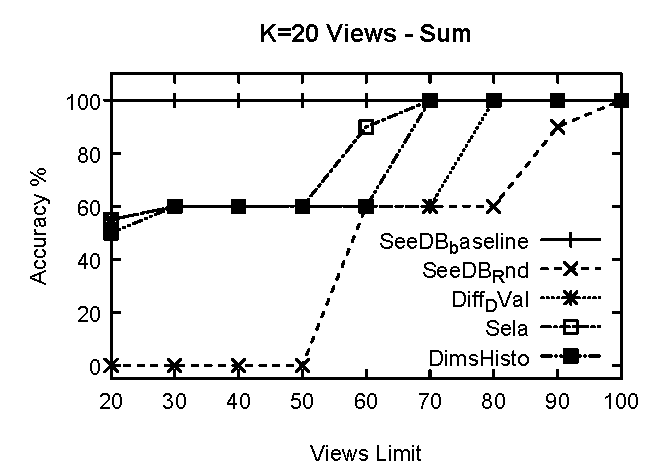
\includegraphics[width=\textwidth]{SumA2.pdf}
    \caption{Sum}
     \label{fig:SumA2}%
  \end{subfigure}
  %
  \begin{subfigure}[b]{0.32\textwidth}
    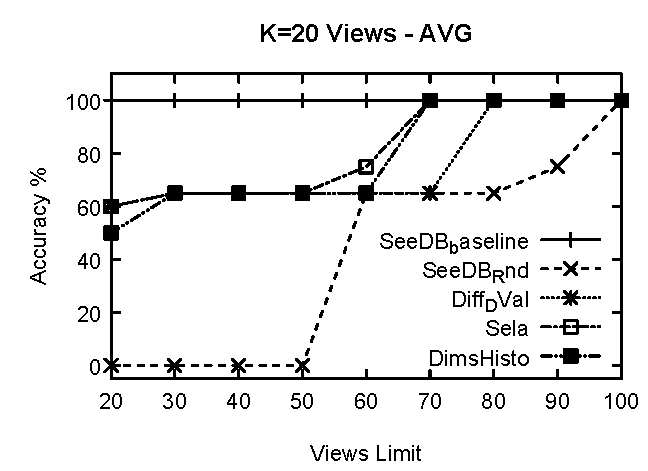
\includegraphics[width=\textwidth]{AvgA2.pdf}
     \caption{Average}
        \label{fig:AvgA2}
  \end{subfigure}
  \begin{subfigure}[b]{0.32\textwidth}
    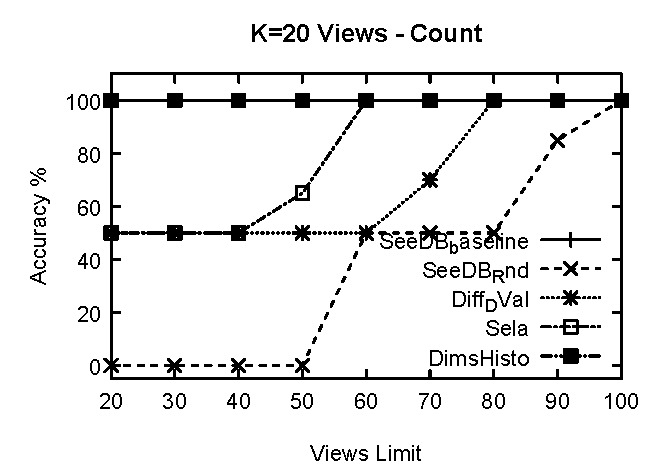
\includegraphics[width=\textwidth]{CountA2.pdf}
     \caption{count}
        \label{fig:CountA2}
  \end{subfigure}
  \caption{Accuracy on varying view space sizes for the Algorithms $Sela$ ,$Diff_DVal$, $DimsHisto$, and $SeeDB_Rnd$}
\end{figure}

\begin{figure}[h]
  \begin{subfigure}[b]{0.32\textwidth}
    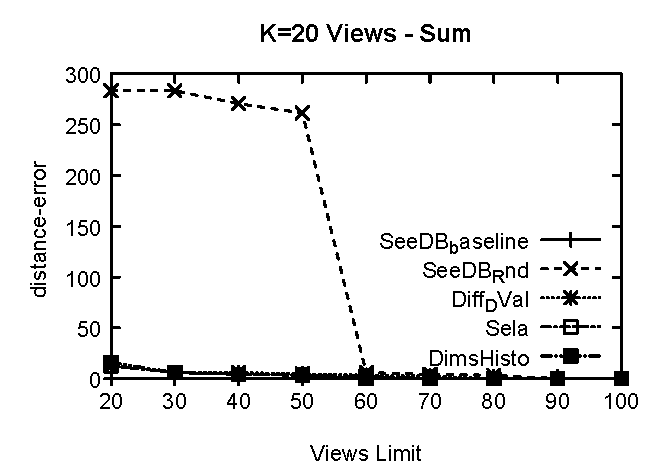
\includegraphics[width=\textwidth]{SumD2.pdf}
    \caption{Sum}
        \label{fig:SumD2}%
  \end{subfigure}
  %
  \begin{subfigure}[b]{0.32\textwidth}
    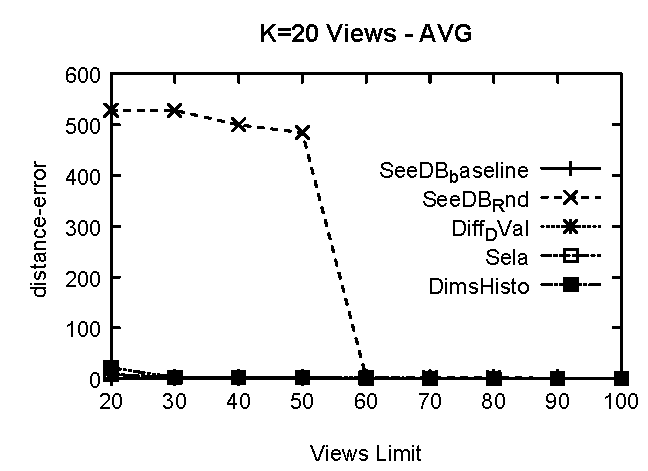
\includegraphics[width=\textwidth]{AvgD2.pdf}
     \caption{Average}
        \label{fig:AvgD2}
  \end{subfigure}
  \begin{subfigure}[b]{0.32\textwidth}
    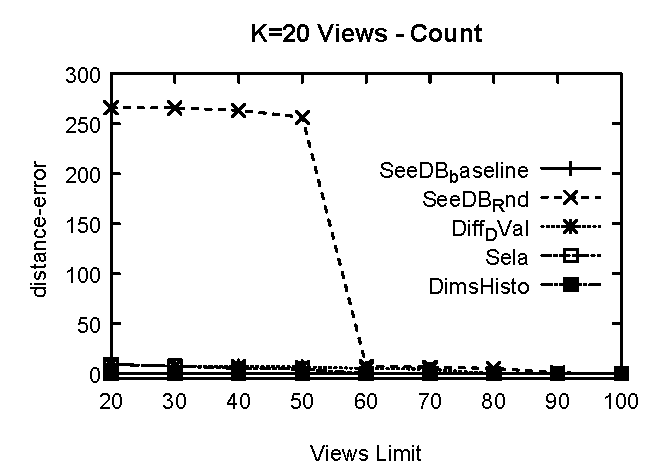
\includegraphics[width=\textwidth]{CountD2.pdf}
     \caption{count}
        \label{fig:CountD2}
  \end{subfigure}
  \caption{Distance-error on varying view space sizes for the Algorithms $Sela$ ,$Diff_DVal$, $DimsHisto$, and $SeeDB_Rnd$}
\end{figure}

As shown in figures \ref{fig:SumD2},\ref{fig:AvgD2},\ref{fig:CountD2} The proposed algorithms produce results near-zero distance-error for all aggregate functions compared with lower baseline strategy $SeeDB_Rnd$ which produce views with low quality however, the quality of the recommended views produced by the proposed algorithms is almost near to the same utilities of views output by the top baseline $SeeDB baseline$. The distance-error of results in the first view limits=20 and 30 views as shown in figures \ref{fig:MaxD2},\ref{fig:MinD2} is high specially for the aggregate function \emph{Min} because functions such as Min and Max are not docile for sampling but the proposed algorithms still score very low distance-error as shown in the figures.
 
 %\begin{center}
  \begin{figure}[h]
  \centering
  \begin{subfigure}[b]{0.42\textwidth}
    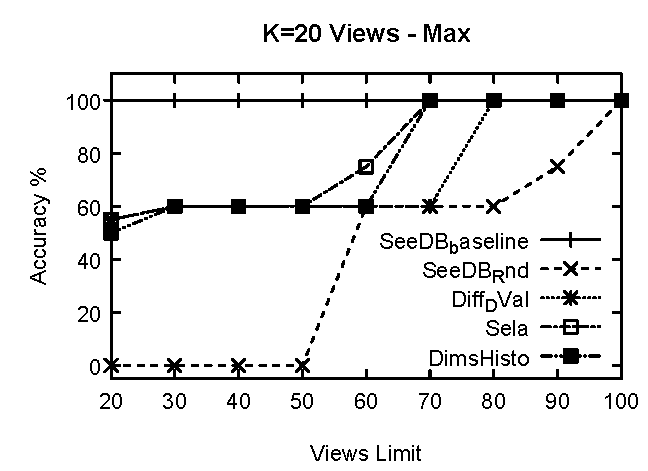
\includegraphics[width=\textwidth]{MaxA2.pdf}
    \caption{Max}
        \label{fig:MaxA2}%
  \end{subfigure}
  %
  \begin{subfigure}[b]{0.42\textwidth}
    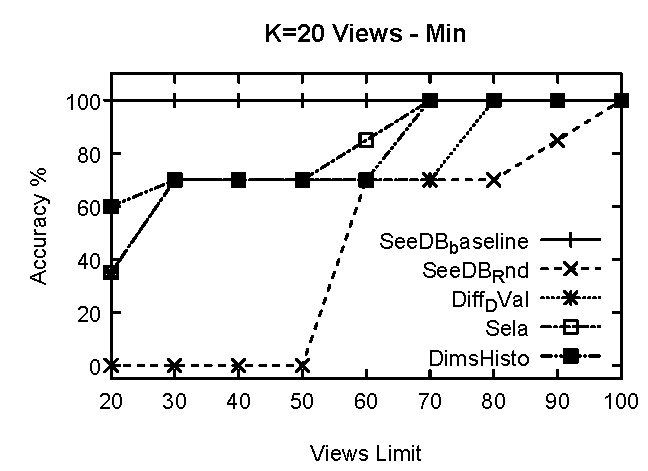
\includegraphics[width=\textwidth]{MinA2.pdf}
     \caption{Min}
        \label{fig:MinA2}
	% \caption{Accuracy on varying view space sizes for the Algorithms $Sela$ ,$Diff_DVal$, $DimsHisto$, and $SeeDB_Rnd$}
  \end{subfigure}
  \caption{Accuracy on varying view space sizes for the Algorithms $Sela$ ,$Diff_DVal$, $DimsHisto$, and $SeeDB_Rnd$}
\end{figure}
%\end{center}

%\begin{center}
  
\begin{figure}[h]
  \centering

  \begin{subfigure}[b]{0.42\textwidth}
    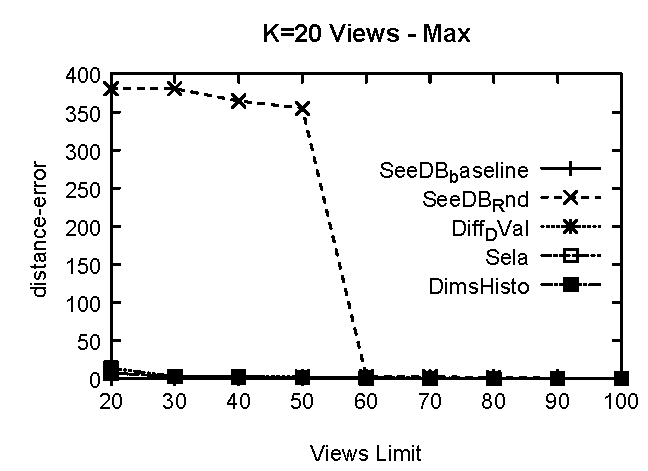
\includegraphics[width=\textwidth]{MaxD2.pdf}
    \caption{Max}
        \label{fig:MaxD2}%
  \end{subfigure}
  %
  \begin{subfigure}[b]{0.42\textwidth}
    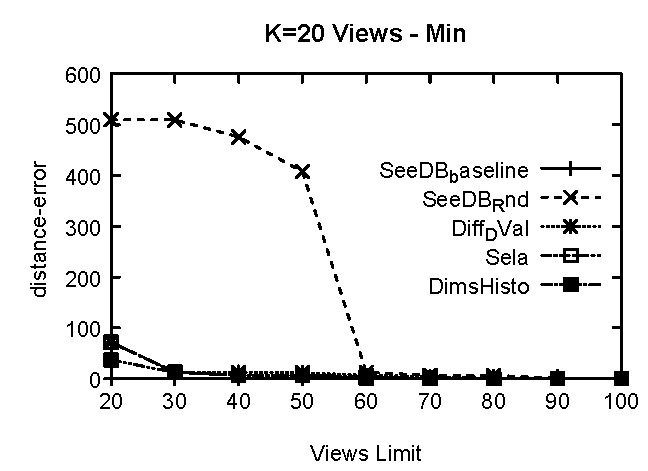
\includegraphics[width=\textwidth]{MinD2.pdf}
     \caption{Min}
        \label{fig:MinD2}
  \end{subfigure}
  
  \caption{Distance-error on varying view space sizes for the Algorithms $Sela$ ,$Diff_DVal$, $DimsHisto$, and $SeeDB_Rnd$}
\end{figure}

%\end{center}

In conclusion, the proposed techniques recommend high quality views in different views limits furthermore, the accuracy is increasing and it doesn't fluctuate along various views limits and similarly the distance-error is declining while increasing the number of explored views (views limit). In the worst cases, the accuracy and the distance-error remain fixed while increasing the number of explored views but they don't decrease. \\
%%%%%%%% Second Expr
\par In the following experiments, we vary $K$ — the number of visualizations
to recommend and fix the number of explored visualizations as \emph{Views Limit=70} and measure the accuracy, and error-distance for each of our
strategies along different aggregate functions. We pay special attention to k = 10 and 20 because empirically these k values are used most commonly.

In summary, $Sela$ and $DimsHisto$ algorithms both produce results with accuracy $100\%$ and zero distance-error when K=10 and 20 views for all aggregate functions as shown in figures \ref{fig:SumA1}, \ref{fig:AvgA1}, \ref{fig:CountA1}, \ref{fig:MaxA1}, and\ref{fig:MinA1} also algorithm $Diff_DVal$ scored accuracy $100\%$ in the first number of recommended views K=10 views. Although, $Diff_DVal$ obtains the same accuracy as $SeeDB_Rnd$ for all aggregate functions but the $Diff_DVal$ scores much better distance-error than $SeeDB_Rnd$ as shown in figures \ref{fig:SumD1}, \ref{fig:AvgD1}, \ref{fig:CountD1}, \ref{fig:MaxD1}, and\ref{fig:MinD1}. As discussed in the previous experiment, the $DimsHisto$ scores accuracy $100\%$ specifically when the aggregate functions \emph{Count} it is also succeeded to recommend views with $100\%$ and zero distance-error for aggregate functions \emph{Sum, Average, and Count} as shown in figures \ref{fig:SumA1}, \ref{fig:AvgA1}, and \ref{fig:CountA1}. In addition, we find that $Sela$ and $DimsHisto$ algorithms produce high quality views with $100\%$ accuracy and zero distance-error for \emph{Max} aggregate function , also they obtain $>75\%$ and $<0.2$ distance error for \emph{Min} aggregate function when k=70 (Views Limit ) as shown in \ref{fig:MaxD1} and \ref{fig:MinD1} receptively.

\begin{figure}[h]
  \begin{subfigure}[b]{0.32\textwidth}
    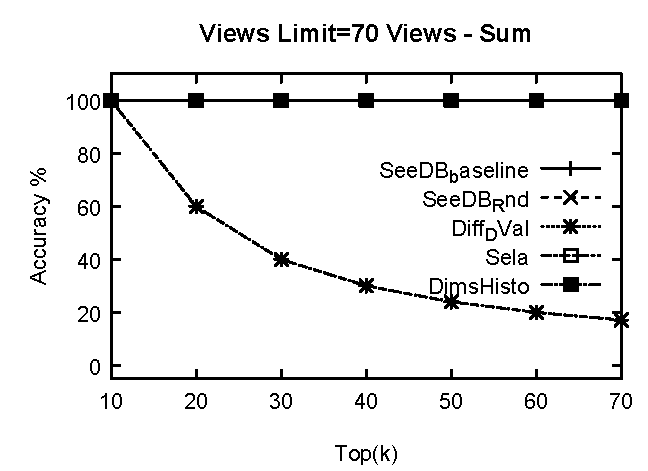
\includegraphics[width=\textwidth]{SumA1.pdf}
    \caption{Sum   }
        \label{fig:SumA1}%
  \end{subfigure}
  %
  \begin{subfigure}[b]{0.32\textwidth}
    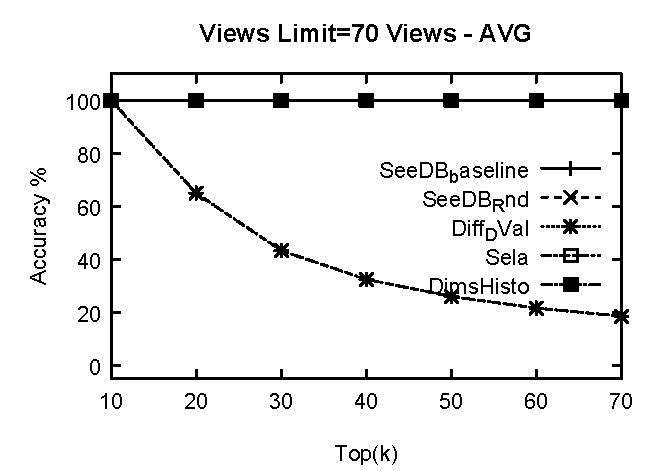
\includegraphics[width=\textwidth]{AvgA1.pdf}
     \caption{Average  }
        \label{fig:AvgA1}
  \end{subfigure}
  \begin{subfigure}[b]{0.32\textwidth}
    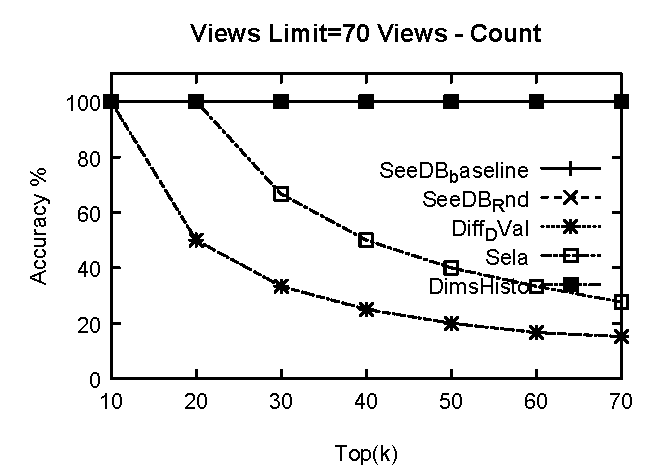
\includegraphics[width=\textwidth]{CountA1.pdf}
     \caption{count  }
        \label{fig:CountA1}
  \end{subfigure}
  \caption{Accuracy on varying view space sizes for the Algorithms $Sela$ ,$Diff_DVal$, $DimsHisto$, and $SeeDB_Rnd$}
\end{figure}

The following figures describe the distance error for the proposed algorithms, we find that although $Diff_DVal$ approach score the same accuracy produced by $SeeDB_Rnd$ strategy but it obtains very low distance error along all aggregate function compared with $SeeDB_Rnd$ strategy as shown in figures \ref{fig:SumD1}, \ref{fig:AvgD1}, \ref{fig:CountD1}, \ref{fig:MaxD1}, and\ref{fig:MinD1}. To Sum up, the proposed approaches boast the accuracy of the recommended views for the mostly common used K values. Moreover, the $Sela$ and $DimsHisto$ achieve better quality results than $Diff_DVal$  because they are capturing the data distribution in the dimension attributes by using selectivity ratios and frequency histograms.
 
\begin{figure}[h]
  \begin{subfigure}[b]{0.32\textwidth}
    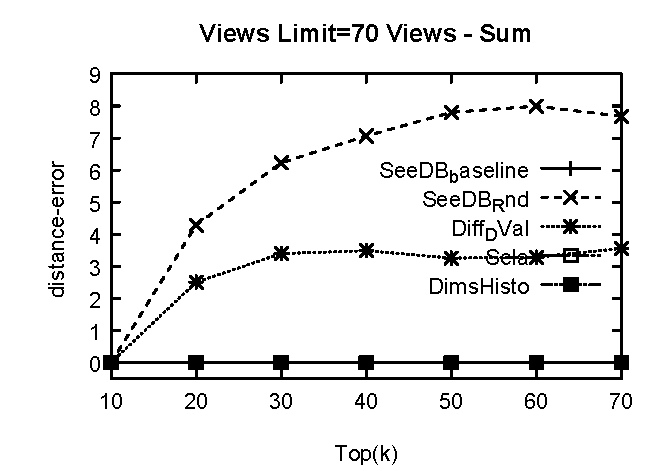
\includegraphics[width=\textwidth]{SumD1.pdf}
    \caption{Sum   }
        \label{fig:SumD1}%
  \end{subfigure}
  %
  \begin{subfigure}[b]{0.32\textwidth}
    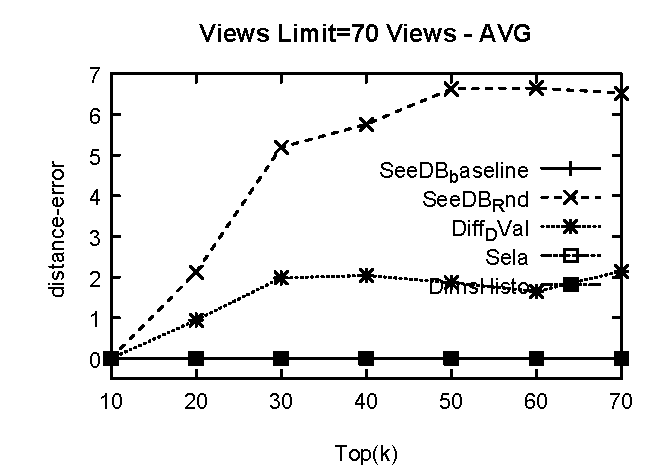
\includegraphics[width=\textwidth]{AvgD1.pdf}
     \caption{Average  }
        \label{fig:AvgD1}
  \end{subfigure}
  \begin{subfigure}[b]{0.32\textwidth}
    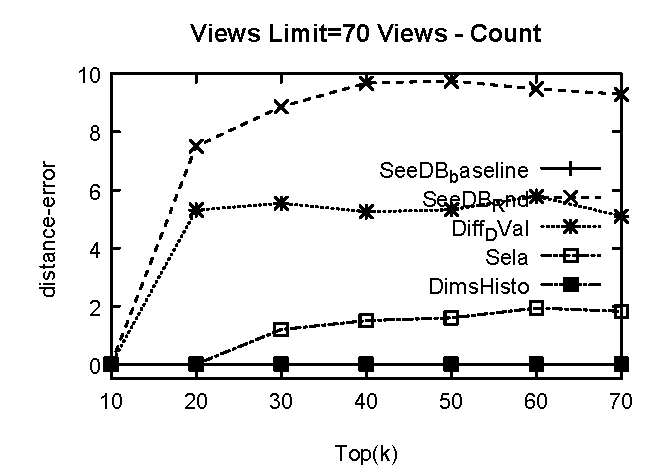
\includegraphics[width=\textwidth]{CountD1.pdf}
     \caption{count  }
        \label{fig:CountD1}
  \end{subfigure}
  \caption{Distance-error on varying k for the Algorithms $Sela$ ,$Diff_DVal$, $DimsHisto$, and $SeeDB_Rnd$}
\end{figure}


 % \begin{center}
    
  \begin{figure}[h]
  \centering
%\end{figure}
  \begin{subfigure}[b]{0.42\textwidth}
    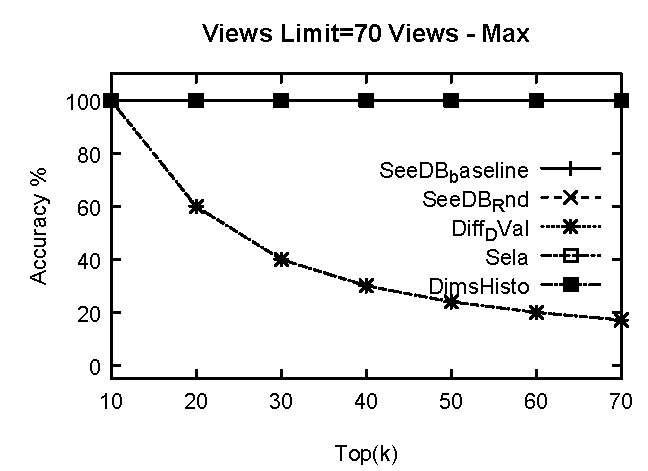
\includegraphics[width=\textwidth]{MaxA1.pdf}
    \caption{Max   }
        \label{fig:MaxA1}%
  \end{subfigure}
  %
  \begin{subfigure}[b]{0.42\textwidth}
    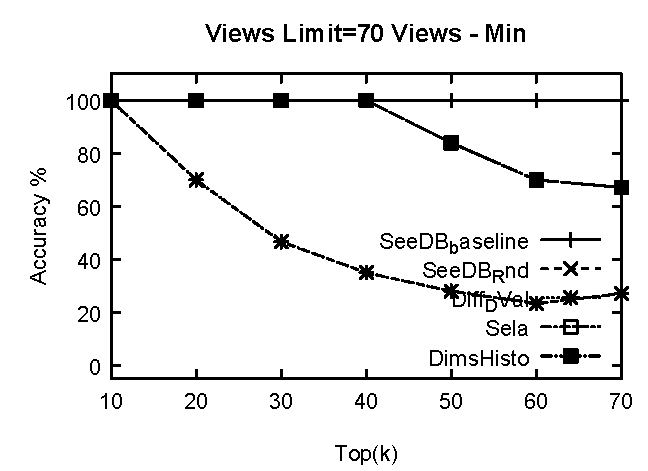
\includegraphics[width=\textwidth]{MinA1.pdf}
     \caption{Min  }
        \label{fig:MinA1}
  \end{subfigure}
  
  \caption{Accuracy on varying K for the Algorithms $Sela$ ,$Diff_DVal$, $DimsHisto$, and $SeeDB_Rnd$}
\end{figure}
%\end{center}

%\begin{center}
  
\begin{figure}[h]
  \centering
  \begin{subfigure}[b]{0.42\textwidth}
    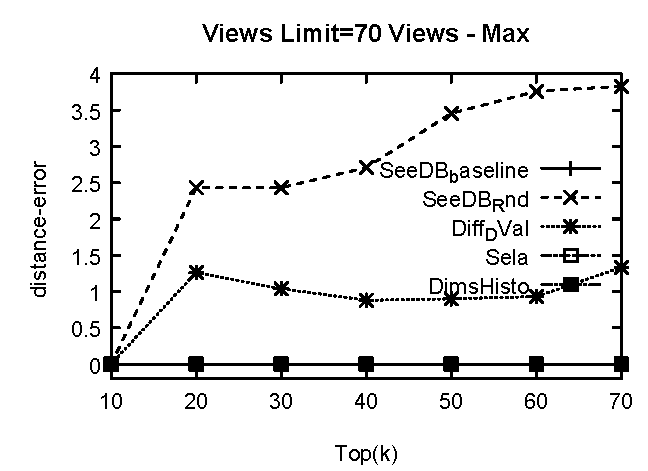
\includegraphics[width=\textwidth]{MaxD1.pdf}
    \caption{Max   }
        \label{fig:MaxD1}%
  \end{subfigure}
  %
  \begin{subfigure}[b]{0.42\textwidth}
    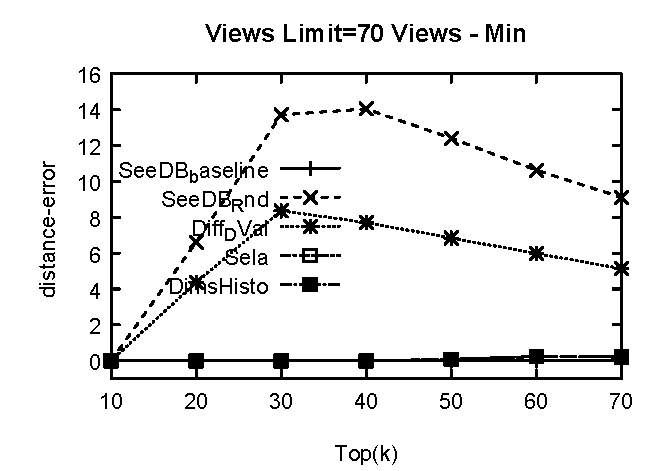
\includegraphics[width=\textwidth]{MinD1.pdf}
     \caption{Min  }
        \label{fig:MinD1}
  \end{subfigure}
  
  \caption{Distance-error on varying K for the Algorithms $Sela$ ,$Diff_DVal$, $DimsHisto$, and $SeeDB_Rnd$}
\end{figure} 

\subsection{Accuracy evaluation}
The dataset used is $GoCard$ data with size 4.4 M tuples contains 9 dimension attributes and 3 measures attributes with we run this experiment on SeeDB over \emph{All} aggregate functions \emph{Count, Sum, Average, Min, and Max} and total of all possible views in each dataset referred as a space size=$5 \times 9 \times 3=135$ views and 
the deviation metric is Earth Movers Distance (EMD). \\ %\mas{what is the input query(s)?} 
\footnotesize {$Q:$ Select * from gocard where alightingstop ='University of Queensland'} 

%\thefontsize 
\normalsize 
%\mas{use straight lines to connect points not curves}
%\mas{use the right accuracy metric}
we implement two baseline strategies. The SeeDB baseline strategy processes the entire data and does not discard any views ($SeeDB baseline$). It thus provides an upper bound on 
latency and accuracy and lower bound on error distance. The other baseline strategy we evaluate is the random strategy ($SeeDB_Rnd$) that returns a random set of k aggregate views as the result. This strategy gives a lower bound on accuracy and upper bound on error distance: for any technique to be useful, it must do significantly better than $SeeDB_Rnd$.
\\ In figure \ref{fig:fig1} shows the accuracy of the results produced by algorithms $Sela$ , $Diff_DVal$, $DimHisto$, and $SeeDB_Rnd$ to find a top $(K=25)$ views
 comparing with different view space sizes. As shown all proposed algorithms  $Sela$ and $Diff_DVal$ scored the same accuracy in the first 30 explored views however, algorithm $DimsHisto$ shows lower accuracy than $Sela$ and $Diff_DVal$ when the number of explored views is 45 because $DimHisto$ evaluates dimension attributes according to their frequencies and it's less descriptive to some aggregate functions such as Max and Min.  Thereafter, the proposed algorithms improve the accuracy to 100\% and keep accuracy stable without any fluctuation.
%\mas{so why it is not doing better when supposedly you proposed it to improve on the first one}
 In addition,  
all proposed algorithms maintain the accuracy of 
results while growing with the extension of the space size while other algorithm 
the accuracy remains stable. Finally, as shown  $SeeDB_Rnd$ is the lowest 
accuracy with different spaces except in the last two space limits. 

\begin{figure}[h]
  \centering
%\end{figure}
  \begin{subfigure}[b]{0.42\textwidth}
    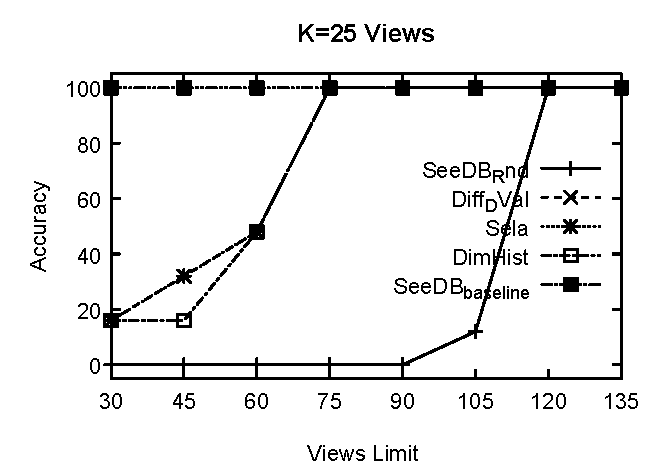
\includegraphics[width=\textwidth]{21.pdf}
    \caption{Accuracy}
        \label{fig:fig1}%
  \end{subfigure}
  %
  \begin{subfigure}[b]{0.42\textwidth}
    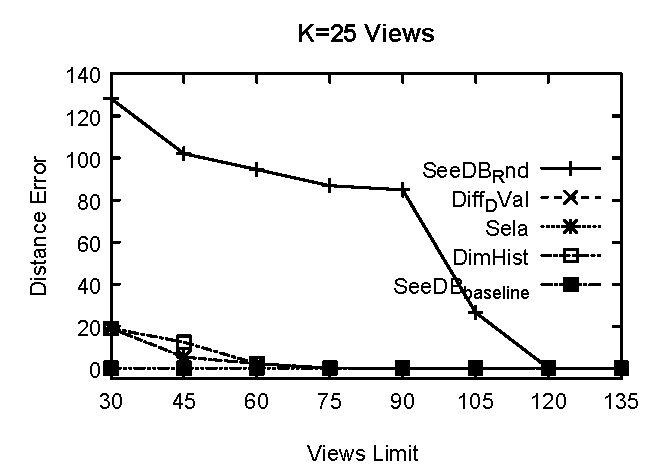
\includegraphics[width=\textwidth]{22.pdf}
     \caption{Error Distance}
        \label{fig:figa2}
  \end{subfigure}
  \caption{Results quality on varying view space sizes for the Algorithms $Sela$ ,$Diff_DVal$, $DimsHisto$, and $SeeDB_Rnd$}
\end{figure}

 %\begin{figure}[h]
%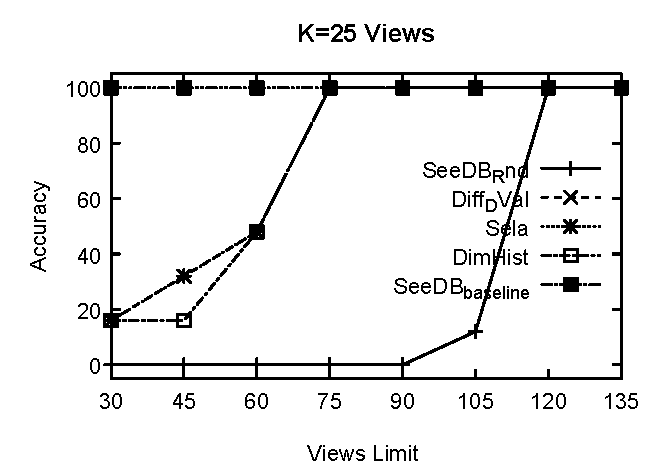
\includegraphics[width=\textwidth]{21.pdf}
%\caption{Accuracy compared with  the view space size for the Algorithms $Sela$ , $N-N'$, $DimHisto$, and $SeeDB_Rnd$}
%\label{fig:fig1}%
%\end{figure}

%\mas{use lines for all and only one y-axis}
In figure \ref{fig:figa2} shows the distance error of the results produced by
algorithms $Sela$ , $Diff_DVal$, and $DimsHisto$ to find a top $(K=25)$ views
 across different number of explored views denoted as 
space sizes as shown algorithms succeeded to minimize the distance error quickly near to $SeeDB Baseline$
specifically when the  
expansion of the space sizes. Although, algorithm $DimsHisto$ obtained lower 
accuracy than $Sela$ and $Diff_DVal$ as shown in figure \ref{fig:fig1} at view space 45, but the 
distance error at the same view space is low because $DimsHisto$ recommended 
different views with high utility distances to minimize the distance error.
%\mas{but supposedly the other two algorithms were two improve on it, but they did not - is that because they are poorly designed or what?}
Other algorithms succeeded to minimize the distance error quickly with 
expansion of the space sizes. 
$SeeDB_Rnd$ shows high distance error even if when the space size is large enough. 
%\begin{figure}[h]
%\includegraphics[width=\textwidth]{{22.pdf}}
%\caption{Error Distance according to the view space size for the Algorithms $Sela$ , $N-N'$, $DimHisto$, and $SeeDB_Rnd$}
%\label{fig:figa2}%
%\end{figure}

%\mas{That is a very shallow comment! You need to explain what happened and why?}
To sum up, the proposed algorithms evaluate the 
dimension attribute according to different priorities methods by recommending set of views 
which improve the quality of the view space limit R in terms of minimizing the distance error and 
enhancing the accuracy as shown in figures \ref{fig:fig1} and  \ref{fig:figa2}.
  
%  \begin{figure}[h]
%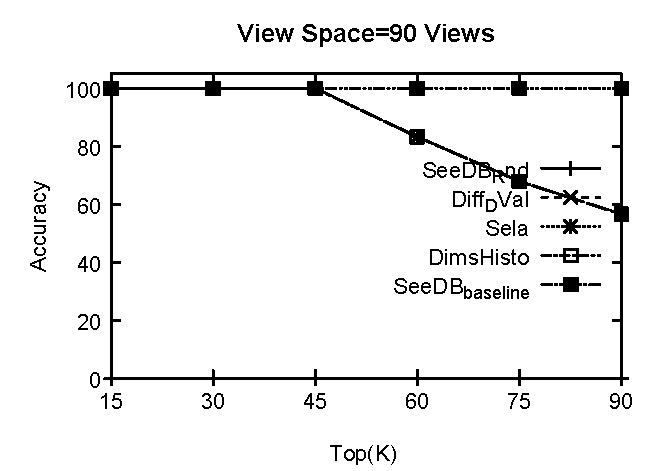
\includegraphics[width=\textwidth]{11.pdf}
%\caption{Accuracy compared with  top(K) views for the Algorithms $Sela$ , $N-N'$, $DimHisto$, and $SeeDB_Rnd$}
%\label{fig:fig3}%
%\end{figure}

\begin{figure}[h]
 \centering
%\end{figure}
  \begin{subfigure}[b]{0.42\textwidth}
    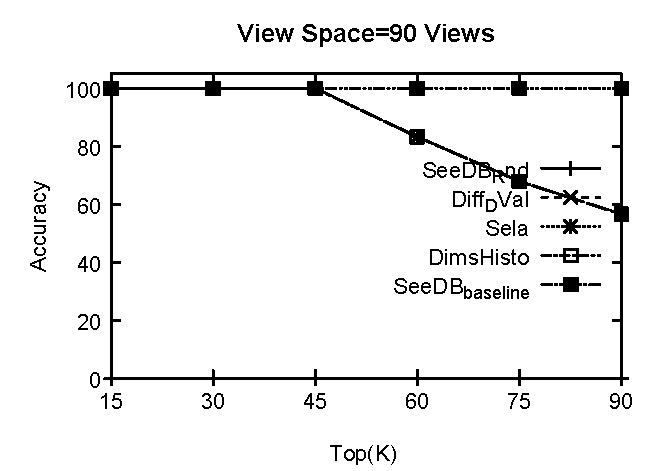
\includegraphics[width=\textwidth]{11.pdf}
    \caption{Accuracy  }
       \label{fig:fig3}
  \end{subfigure}
  %
  \begin{subfigure}[b]{0.42\textwidth}
    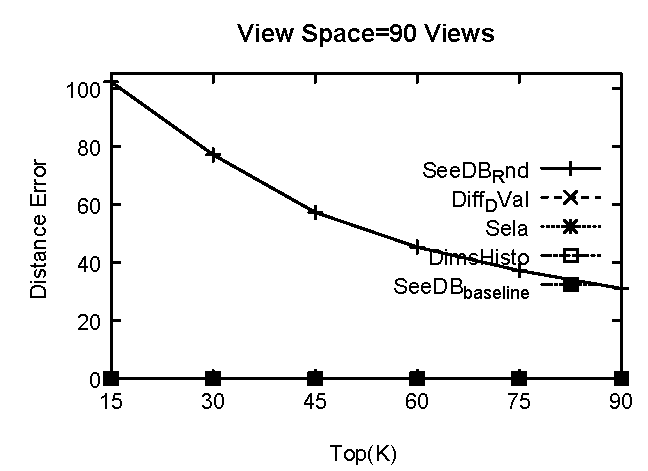
\includegraphics[width=\textwidth]{12.pdf}
     \caption{Error Distance  }
       \label{fig:fig4}%
  \end{subfigure}
  \caption{Results quality on varying top(K) views for the Algorithms $Sela$ , $Diff_DVal$, $DimHisto$, and $SeeDB_Rnd$}
\end{figure}

In figure \ref{fig:fig3} shows the accuracy of the 
algorithms $Sela$ , $Diff_DVal$, $DimsHisto$, and $SeeDB_Rnd$ in a fixed space size $R=90$ views
 comparing with different view 
space top(k) views as shown all algorithms scored 100\% accuracy in the first top 45 views 
which form half number of explored views.
We observe that the accuracy declines 
%\mas{why is that?!!} 
while increasing top(K) in a fixed space limit. 
This because wrong priortrizing of one dimension attribute than another will consequently affects on all 
recommended views that created from the wrong dimension attribute. However, the accuracy is above
50\% when k=90 (the entire view space limit) as shown in figure \ref{fig:fig3}. 
Furthermore, the analyst is usually interested in recommending a small number of 
visualisations e.g. k=25. 
%\begin{figure}[t]
%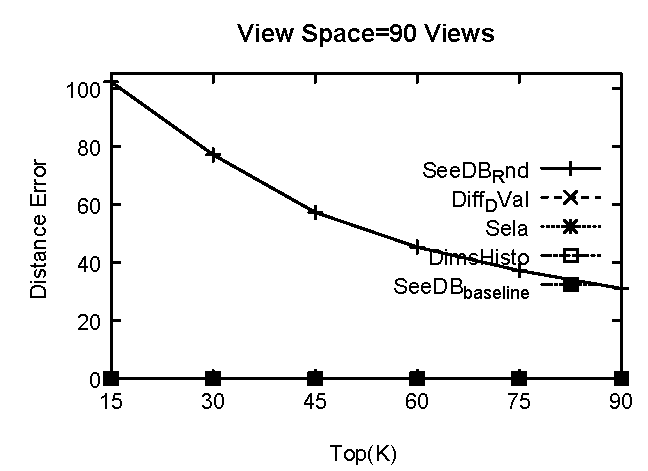
\includegraphics[width=\textwidth]{12.pdf}
%\caption{Error Distance compared with  the view space size for the Algorithms $Sela$ , $N-N'$, $DimHisto$, and $SeeDB_Rnd$}
%\label{fig:fig4}%
%\end{figure}

%\mas{again, what you proposed as better algorithms, performed worse than the basic one, why?!}
In figure \ref{fig:fig4} shows the distance error  of the 
algorithms $Sela$ , $Diff_DVal$, $DimHisto$, and $SeeDB_Rnd$ in a fixed space size $R=150$ views
 comparing with different Top(K) views 
 all algorithms have a very small distance error $\approx 0$ for Top(60) views
 however, $Diff_DVal$algorithm 
shows the smallest distance error across different K sizes. Both $Sela$  and $DimHisto$ 
report growing rise in the distance error with respect to Top(K) views required 
by the user in the certain view space size=90 views.\\

 In conclusion, the discussed algorithms $Sela$ ,$Diff_DVal$, $DimHisto$ show high 
 accuracy and low distance errors along different space sizes and 
 varying Top(K) as  illustrated previously however,
  these algorithms differentiate on the quality measures .For instance, 
 algorithm $Sela$ and $Diff_DVal$ 
 gain the highest accuracy than $DimHisto$ in the experiments as shown in
 figures  \ref{fig:fig1} and \ref{fig:fig3} but algorithm $Diff_DVal$  has the lowest error distance as shown in figures  \ref{fig:figa2} and \ref{fig:fig4}. 
 %
 \subsection{Efficiency evaluation}
  In this section, we evaluated the efficiency of the prioritizing algorithms in terms of the execution overhead added to 
	SeeDB (as automatic recommendation engine) by computing the costs of executing the proposed algorithms and gains of applying 
	the algorithms. Similarly, as the previous experiments, we measured the efficiency the algorithms 
	by running experiments to capture the overhead and the gains 
	along different $Top(K)$ and varying space limits compared with the actual execution of SeeDB baseline. 
 All the experiments were repeated 5 times and the measurements were averaged. We begin by presenting a summary of our experimental
findings and then dive into performance results for individual optimizations.

we compared the executions costs of the algorithms added to SeeDB with the original 
baseline of SeeDB to identify the improvements in the performance. As
shown in figure \ref{fig:fig33} shows the total SeeDB and algorithms execution 
times compared with the original SeeDB baseline. This figure shows the improvements
in the SeeDB performance with different space limits to find a top (K = 25) views. 
As shown the 
improvements in the performance by using the proposed algorithms 
are significant compared with the baseline furthermore, the execution costs increase linearly 
with the view space limit produced by algorithms. 
%\mas{what happens after 120? do the other two also exceed SeeDB?}
\begin{figure}
   \centering
%\end{figure}
  \begin{subfigure}[b]{0.42\textwidth}
    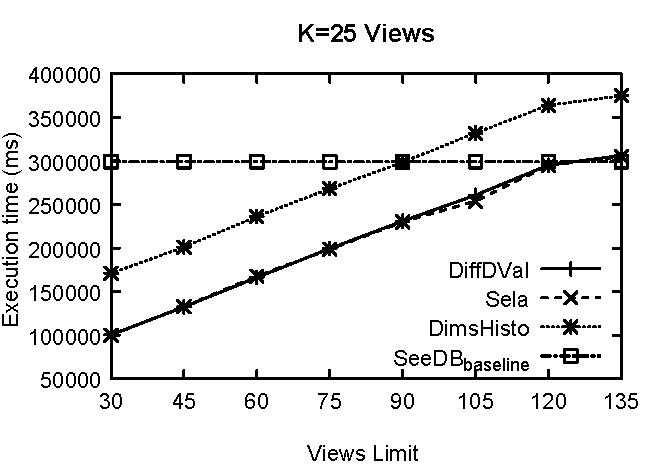
\includegraphics[width=\textwidth]{33.pdf}
    \caption{Execution times of algorithms across views limits}
    \label{fig:fig33}
  \end{subfigure}
  %
  \begin{subfigure}[b]{0.42\textwidth}
    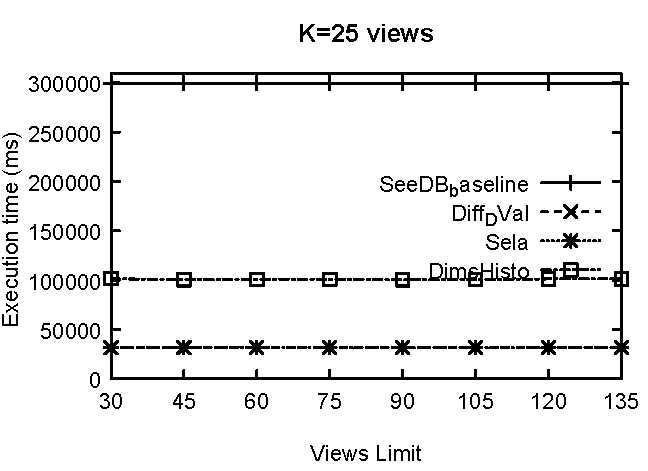
\includegraphics[width=\textwidth]{34.pdf}
    \caption{The overhead costs of proposed algorithms}
    \label{fig:fig34}
  \end{subfigure}
  \caption{Algorithms Performance on different space limits}
\end{figure}

%\mas{very confusing plot! what are the different components? and what are they stacked on top of each other?}
In Figure \ref{fig:fig34} illustrates the executions times of the 
algorithms $Sela$ , $Diff_DVal$ and $DimsHisto$ across different space limits 
however, this cost is considered as extra overhead should be added. As presented 
the executions times of the algorithms are almost stable along different space sizes 
because the algorithms evaluate a fixed set of dimension attributes every time. 
However, algorithm $DimsHisto$ is costly as it poses same number of queries to create histograms
then it computes the distance among those histograms.\\

\begin{figure}
   \centering
%\end{figure}
  \begin{subfigure}[b]{0.42\textwidth}
    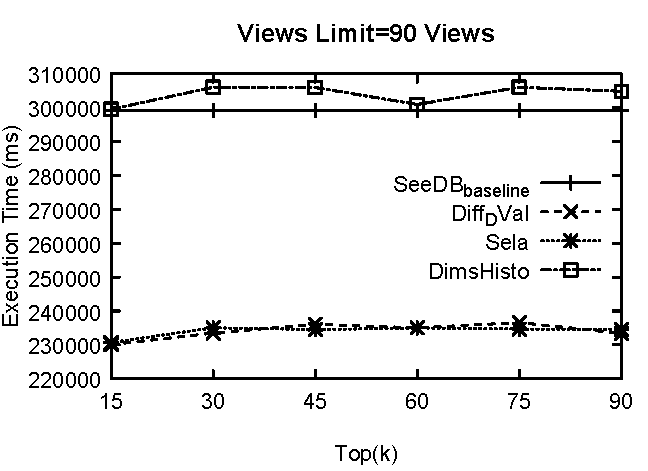
\includegraphics[width=\textwidth]{31.pdf}
    \caption{Total Execution time of the algorithms on fixed space limit}
    \label{fig:fig31a}
  \end{subfigure}
  %
  \begin{subfigure}[b]{0.42\textwidth}
    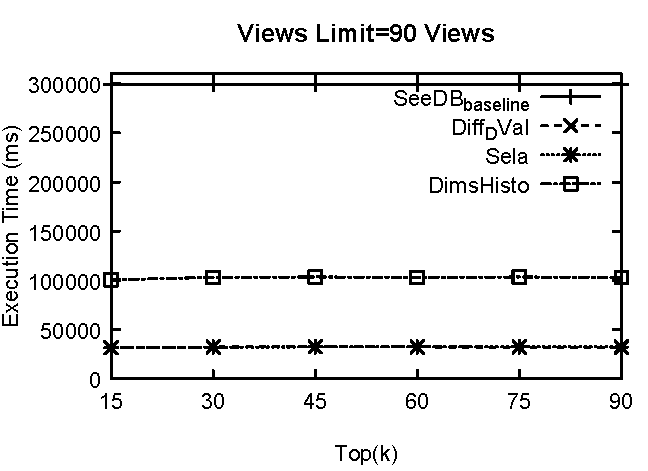
\includegraphics[width=\textwidth]{32.pdf}
    \caption{Overhead costs of the algorithms on fixed space limit}
    \label{fig:fig32}
  \end{subfigure}
  \caption{Algorithms Performance on varying $Top(k)$ views}
\end{figure}

The following figures discuss the efficiency of the proposed algorithms along different 
$Top(K)$ views in a certain space limit=90. As shown in figure 
\ref{fig:fig31a}, the proposed algorithms show improvements in the execution more 
than 40\% compared with the SeeDB baseline execution time. As discussed earlier, 
algorithm $DimsHisto$ shows the highest cost among algorithms $Sela$ and $Diff_DVal$. 
In other hand, figure \ref{fig:fig32} describes the execution costs of the algorithms separately. 
The running costs of algorithms are fixed while expanding $K$ the number of top deviated views 
because the algorithms run on a specified 
space limit.




 
\input{Expertl}
\section{Related Work}
\label{sec:related}
%
Interactive Data Visualization Tools: have interested the research community over the past few years, and it has presented a number of interactive data analytics tools such as ShowMe, Polaris, and Tableau \cite{kandel2012profiler,DBLP:journals/tvcg/MackinlayHS07,DBLP:conf/sigmod/KeyHPA12,DBLP:journals/tvcg/Fisher07}. 
%
Similar visualization specification tools have also been introduced by the database community, including Fusion Tables \cite{DBLP:conf/sigmod/GonzalezHJLMSSG10} and the Devise \cite{DBLP:conf/sigmod/LivnyRBCDLMW97} toolkit. 
%
Unlike SeeDB, which recommends visualizations automatically by exploring the entire views space, these tools place the onus on the analyst to specify the visualization to be generated. For datasets with a large number of attributes, it is unfeasible for the analyst to manually study all the attributes; hence, interactive visualization needs to be augmented with automated visualization techniques.
%

A few recent systems have attempted to automate some aspects of data analysis and visualization. Profiler is one such automated tool that allows analysts to detect anomalies in data \cite{kandel2012profiler}. Another related tool is VizDeck \cite{DBLP:conf/sigmod/KeyHPA12}, in given a dataset, depicts all possible 2-D visualizations on a dashboard that the user can control by reordering or pinning visualizations. Given that VizDeck generates all visualizations, it is only meant for small datasets; and VizDeck does not discuss techniques to speed-up the generation of these visualizations.
%

To support visual sense-making in medical diagnosis, INVISQUE\cite{Wong2011,DBLP:conf/chi/WongCKRX11} is an interactive visualization system proposed such as physical index cards on a two dimensional
workspace. INVISQUE provides some features to support ‘annotating, re-visiting, and merging two clusters. It discusses essential problems in designing medical diagnostic displays that can improving the review of a patient’s medical history \cite{Wong2011}. A recent work, SubVIS \cite{Hund2016} is a visualization tool which assists the user to analyze and interactively explore computed subspaces to discover insights in highly dimensional and complex patient's datasets. SubVIS \cite{Hund2016} introduces an analysis workflow to visually explore subspace clusters from various perspectives and it tackles some subspace clustering challenges such as difficulty of interpretation patient results, redundancy detection in subspaces and clusters, and multiple clustering results for different parameter settings.    
%

Statistical analysis and graphing packages such as R, SAS and Matlab could also be used generate visualizations, but they lack the ability to filter and recommend 'interesting' visualizations.
%

OLAP: there has been some work on browsing data cubes, allowing analysts to variously find \emph{explanations} for why two cube values were different, to find which neighboring cubes have similar properties to the cube under consideration, or get suggestions on what unexplored data cubes should be looked at next \cite{DBLP:journals/dr/Jagadish99b,DBLP:conf/vldb/Sarawagi00,DBLP:conf/vldb/SatheS01}.
%

Database Visualization Work: Fusion tables \cite{DBLP:conf/sigmod/GonzalezHJLMSSG10} allow users to create visualizations layered on top of web databases; they do not consider the problem of automatic visualization generation. Devise \cite{DBLP:conf/sigmod/HellersteinHW97} translated user-manipulated visualizations into database queries.
%

Although the aforementioned approaches provide assistance in query visualization, they lack the ability to automatically recommend interesting visualizations, except SeeDB which provides different optimization techniques to automatically recommend interesting visualizations while avoiding unnecessary visualizations by utilizing two kinds of optimization techniques as explained next.\\
%

\noindent \textbf{Visualizations Pruning in SeeDB:}
SeeDB implement an execution engine to reduce latency in assessing the collection of 
aggregate views which it applies two kinds of optimizations: sharing, 
where aggregate view queries are combined to share computation as much as possible, 
and pruning, where aggregate view queries corresponding to low utility visualizations 
are dropped from consideration without scanning the whole dataset. 
SeeDB developed a phased execution framework,each phase operates on a subset of the dataset. 
Phase i of n operates on the $i^{th}$ of n equally-sized partitions of the dataset. 
%(Empirically, we have found n = 10 to work well, though our results are not very sensitive to the value of n.) 
%For instance, if we have 100, 000 records and 10 phases, the i = 4th phase 
%processes records 30, 001 to 40, 000. 
The execution engine begins with the entire set of aggregate views as follows:
� During phase i,the SeeDB \cite{DBLP:journals/pvldb/VartakMPP14} modifies partial results for the views still under consideration 
using the $i^{th}$ fraction of the dataset. 
The execution engine applies sharing-based optimizations to minimize scans on this $i^{th}$ fraction 
of the dataset.
� At the end of phase i,the execution engine uses pruning-based optimizations to determine which aggregate views to discard. The partial results of each aggregate view on the fractions from 1 through i are used to estimate the quality of each view, and the views with low utility are discarded.

The execution engine uses pruning optimizations to determine 
which aggregate views to discard. Specifically, partial results for each 
view based on the data processed so far are used to estimate utility and views 
with low utility are discarded. SeeDB execution engine supports two pruning schemes. 
The first uses confidence-interval techniques to bound utilities of views, while the second 
uses multi-armed bandit allocation strategies to find top utility views.\\
 \begin{itemize}
\item {Confidence Interval-Based Pruning:} The first pruning scheme uses worst-case statistical confidence intervals to bound views utilities. 
 This technique is similar to top-k based pruning algorithms developed in other contexts \cite{serfling1974probability}. 
 It works as follows: during each phase, 
 it keeps an estimate of the mean utility for every aggregate view $V_i$ and a confidence 
 interval around that mean. At the end of a phase, it applies the following rule to 
 prune low-utility views: If the upper bound of the utility of view $V_i$ is less than the lower bound 
 of the utility of k or more views, then $V_i$ is discarded. 
\item {Multi-Armed Bandit Pruning:} Second pruning scheme employs a Multi-Armed Bandit strategy (MAB)
\cite{DBLP:journals/pvldb/VartakMPP14,DBLP:conf/icml/BubeckWV13}. 
In MAB, an online algorithm repeatedly chooses from a set of alternatives over 
a sequence of trials to maximize reward. 
This variation is identical to the problem addressed by SeeDB: the goal is find the 
visualizations (arms) with the highest utility (reward). 
Specifically, SeeDB adapts the Successive Accepts and Rejects algorithm from \cite{DBLP:conf/icml/BubeckWV13}
to find arms with the highest mean reward. At the end of every 
phase, views that are still under consideration are ranked in order of their 
utility means. We then compute two differences between the utility means: $\Delta {1} $is the difference 
between the highest mean and the $k + 1^{st}$ highest mean, and $\Delta{n}$ is the difference between 
the lowest mean and the ${k}^{th}$ highest mean. If $\Delta {1}$ is greater than $ \Delta{n}$, the view with the 
highest mean is �accepted� as being part of the top-k (and it no longer participates in pruning computations). 
On the other hand, if $ \Delta{n}$ is higher, the view with the lowest mean is discarded from the set of 
views in the running. [6] proves that under certain assumptions about reward distributions, 
the above technique identifies the top-k arms with high probability.
 
\end{itemize}
 
 However, SeeDB pruning schemes experience some limitations, as they assume 
  fixed data distribution  \cite{DBLP:journals/pvldb/VartakMPP14,vartakseedb}  for sampling to estimate
  the utility of views and require large samples for pruning low utility views with high guarantees.
  Moreover, aggregate functions MAX and MIN are not docile to sampling-based 
  optimizations. \\
	
\noindent \textbf {Offline visualizations in SeeDB: }
SeeDB prunes redundant views \cite {DBLP:journals/pvldb/VartakMPP14} : (1) For each table, it first determines 
the entire space of aggregate views. (2) Next, it prunes all 
aggregate views containing attributes with 0 or low variance since corresponding 
visualizations are unlikely to be interesting. (3) For each remaining view $V_i$, SeeDB computes
 the distribution for reference views on the entire dataset . 
 (4) The resulting distributions are then clustered based on pairwise correlation. 
 (5) From each cluster, SeeDB selects one view to compute as a cluster representative and 
 store �stubs� of clustered views for sub- sequent use. At run time, the view generator accesses 
 previously generated view stubs, removes redundant views and passes the remaining stubs 
 to the execution engine. 

\section{Conclusion}
%
Finding top interesting visualizations by exploring a specified number of visualizations or an execution time budget, while persevering the quality and the accuracy of the recommended views is a challenging and emerging problem. 
%
In this paper, we addressed this problem and proposed an efficient framework called Realtime Scoring Engine (RtSEngine) that assist data analysts in the exploration of visualizations generated from structured databases.
%

Specifically, RtSEngine supports analysts by efficiently recommending visualizations while meeting analyst’s budgets: certain number of visualizations or execution time quote.
%
%to limit the exploration of visualizations for a specified number of visualizations or certain execution time quote to recommend a set of views that meets the analyst’s budgets. 
%
RtSEngine accomplishes this by incorporating inventive approaches to prioritize and score attributes that form all possible visualizations in database based on their statistical proprieties such as selectivity ratio, data distribution, and number of distinct values.
%
Then, RtSEngine recommends the views created from top scored attributes.
%

In addition, we presented visualizations cost-aware techniques that estimate the retrieval and computation costs of all visualizations.
%
Those estimated costs are then fed to RtSEngine to recommend views while considering their costs to guarantee the efficiency and effectiveness of the recommendation process. 
%
%
% utilise the estimated costs with to recommend views while considering their costs. 
%

Finally, we conducted comparative experiments and demonstrated the quality of visualizations and the overhead obtained by applying our techniques on both synthetic and real datasets.
%
The experiments showed superior effectiveness and efficiency of our proposed approaches on different time and space limits. 
%
%\section{Section title}
%\label{sec:1}
%Text with citations \cite{RefB} and \cite{RefJ}.
%\subsection{Subsection title}
%\label{sec:2}
%as required. Don't forget to give each section
%and subsection a unique label (see Sect.~\ref{sec:1}).
%\paragraph{Paragraph headings} Use paragraph headings as needed.
%\begin{equation}
%a^2+b^2=c^2
%\end{equation}
%
 %For one-column wide figures use
%\begin{figure}
 %Use the relevant command to insert your figure file.
 %For example, with the graphicx package use
  %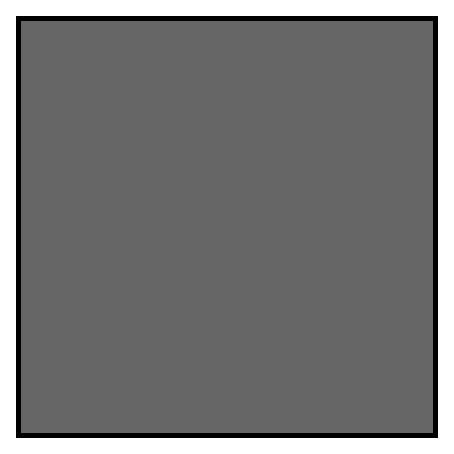
\includegraphics{example.eps}
 %figure caption is below the figure
%\caption{Please write your figure caption here}
%\label{fig:1}       % Give a unique label
%\end{figure}

 %For two-column wide figures use
%\begin{figure*}
 %Use the relevant command to insert your figure file.
 %For example, with the graphicx package use
  %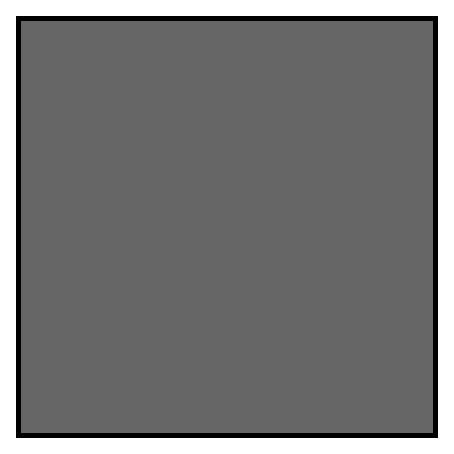
\includegraphics[width=0.75\textwidth]{example.eps}
 %figure caption is below the figure
%\caption{Please write your figure caption here}
%\label{fig:2}       % Give a unique label
%\end{figure*}

 %For tables use
%\begin{table}
 %table caption is above the table
%\caption{Please write your table caption here}
%\label{tab:1}       % Give a unique label
 %For LaTeX tables use
%\begin{tabular}{lll}
%\hline\noalign{\smallskip}
%first & second & third  \\
%\noalign{\smallskip}\hline\noalign{\smallskip}
%number & number & number \\
%number & number & number \\
%\noalign{\smallskip}\hline
%\end{tabular}
%\end{table}


%\begin{acknowledgements}
%If you'd like to thank anyone, place your comments here
%and remove the percent signs.
%\end{acknowledgements}

% BibTeX users please use one of
%\bibliographystyle{spbasic}      % basic style, author-year citations
%\bibliographystyle{spmpsci}      % mathematics and physical sciences
%\bibliographystyle{spphys}       % APS-like style for physics
%\bibliography{}   % name your BibTeX data base
\bibliographystyle{spmpsci} 
%\bibliographystyle{spbasic} 
\bibliography{paper}
% Non-BibTeX users please use

%
%\begin{thebibliography}{}
%
 %and use \bibitem to create references. Consult the Instructions
 %for authors for reference list style.
%
%\bibitem{RefJ}
 %Format for Journal Reference
%Author, Article title, Journal, Volume, page numbers (year)
 %Format for books
%\bibitem{RefB}
%Author, Book title, page numbers. Publisher, place (year)
 %etc
%\end{thebibliography}

\end{document}
% end of file template.tex

